\documentclass{article} % For LaTeX2e
\usepackage{nips13submit_e,times}
\usepackage{hyperref}
\usepackage{url}
\usepackage{amsmath}
\usepackage{graphicx}
\usepackage{booktabs}
\usepackage[raggedright]{sidecap}

% http://www.latex-community.org/forum/viewtopic.php?f=45&t=12364
\sidecaptionvpos{figure}{c}

\title{Language learning via recursive pragmatic reasoning}
% \title{Learning words via recursive pragmatic reasoning about other agents}
% : The blessing of social anxiety - not a huge fan of colon titles

\author{
Nathaniel J.~Smith\thanks{...} \\
School of Informatics\\
University of Edinburgh\\
Edinburgh, Scotland, UK\\
\texttt{nathaniel.smith@ed.ac.uk} \\
\AND
Noah D.~Goodman \\
Department of Psychology\\
Stanford University \\
Stanford, CA, USA \\
\texttt{ngoodman@stanford.edu} \\
\And
Michael C.~Frank \\
Department of Psychology \\
Stanford University \\
Stanford, CA, USA \\
\texttt{mcfrank@stanford.edu}}

\newcommand{\fix}{\marginpar{FIX}}
\newcommand{\new}{\marginpar{NEW}}

\newcommand{\word}{\text{word}}
\newcommand{\obj}{\text{object}}
\newcommand{\lex}{\text{lexicon}}
%\newcommand{\prior}{P_{\text{prior}}(\obj | \text{context})}
\newcommand{\prior}{P_{\text{prior}}(\obj)}


% \nipsfinalcopy % Uncomment for camera-ready version

% Tell LaTeX to break pages in the middle of displayed math whenever
% this would be the slightest bit useful
\allowdisplaybreaks[4]

\begin{document}
\maketitle

\begin{abstract}
  Language users are remarkably good at making inferences about
  speakers' intentions in context, and children learning their native
  language also display substantial skill in acquiring the
  meanings of unknown words. These two cases are deeply related:
  Language users invent new terms in conversation, and language
  learners learn the literal meanings of words based on their
  pragmatic inferences about how those words are used. 
 While pragmatic inference and word
  learning have both been independently characterized in probabilistic
  terms, no current work unifies these two. We describe a
  model in which language learners assume that they jointly
  approximate a shared, external lexicon and reason recursively about
  the goals of others in using this lexicon. This model captures
  phenomena in word learning and pragmatic inference; it additionally
  leads to insights about the emergence of communicative systems in
  conversation and the mechanisms by which pragmatic inferences become
  incorporated into word meanings.
\end{abstract}

\section{Introduction}

Two puzzles present themselves to language users: What do words mean in general and what do they mean in context?
%Natural language is a powerful tool for conveying meaning in context. 
Consider the utterances
``it's raining,'' ``I ate some of the cookies,'' or ``can you close
the window?'' In each, a listener must go beyond the literal meaning
of the words to fill in contextual details (``it's raining here and
now''), infer that a stronger alternative is not true (``I ate some
but not all of the cookies''), or more generally infer the speaker's
communicative goal (``I want you to close the window right now because
I'm cold''), a process known as \textit{pragmatic reasoning}. Theories of pragmatics frame
the process of language comprehension as inference about the
generating goal of an utterance given a rational speaker
\cite{grice1975,dale1995,frank2012}. For example, a listener might
reason, ``if she had wanted me to think `all' of the cookies, she
would have said `all'---but she didn't. Hence `all' must not be true
and she must have eaten some {\it but not all} of the cookies.'' This kind of reasoning is core to language use. 

But pragmatic reasoning about meaning-in-context relies on stable literal meanings that must  themselves be learned.
%and often intersects with learning the meaning of language in general. 
In both adults and children, uncertainty about word meanings is
common, and often considering speakers' pragmatic goals can help to resolve this uncertainty. For example,
if a novel word is used in a context containing both a novel and a
familiar object, young children can make the inference
that the novel word refers to the novel object \cite{markman1988}.\footnote{Very young children
  make inferences that are often labeled as ``pragmatic'' in that they
  involve reasoning about context \cite{clark1988,baldwin1993}, though
  they also show weaknesses in specific inferences (e.g.~strengthening
  {\sc some} to {\sc some but not all} \cite{papafragou2003}). Here we
  remain agnostic about the age at which children are able to make
  such inferences robustly, as it may vary depending on the linguistic
  materials being used in the inference \cite{barner2011}.} For adults
who are proficient language users, there are also a variety of intriguing cases
in which listeners seem to create situation- and task-specific ways of
referring to particular objects. For example, when asked to refer to
idiosyncratic geometric shapes, over the course of an experimental
session, participants create conventionalized descriptions that allow
them to perform accurately even though they do not begin with a shared
label \cite{krauss1964,clark1986}. In both of these examples, reasoning about another person's goals informs language learners' estimates of what words are likely to mean. 

% Recursive pragmatic inferences such as those described above could be
% an important part of language learning. For
% example, the disambiguation inference described above can emerge from
% such reasoning (``why would the speaker have said ``dax'' if there was
% a word for the known object that she knew I would know'')
% \cite{clark1988}.Yet models of grounded language
% learning have failed to take pragmatic factors into account.

Despite this intersection, there is relatively little work that takes pragmatic reasoning into account when considering language learning in context. Recent work on grounded language learning has attempted to learn large sets of (sometimes relatively complex) word meanings directly from corpus data
(e.g.~\cite{zettlemoyer2005,chen2008,frank2009,kwiatkowski2010,johnson2012}). And
a number of models have begun to formalize the consequences of
pragmatic reasoning in situations where limited learning takes place
\cite{golland2010,frank2012,bergen2012}. But as yet these two strands
of research have not been brought together so that the implications of
pragmatics for learning can be investigated directly.


% \footnote{Very young children
%   make inferences that are often labeled as ``pragmatic'' in that they
%   involve reasoning about context \cite{clark1988,baldwin1993}, though
%   they also show weaknesses in specific inferences (e.g.~strengthening
%   {\sc some} to {\sc some but not all} \cite{papafragou2003}). Here we
%   remain agnostic about the age at which children are able to make
%   such inferences robustly, as it may vary depending on the linguistic
%   materials being used in the inference \cite{barner2011}.}

The goal of our current work is to investigate the possibilities for
integrating models of recursive pragmatic reasoning with models of
language learning, with the hope of capturing phenomena in both
domains. We begin by describing previous models in each domain as well
as proposals for bringing the two together. We next simulate findings
on pragmatic inference in one-shot games (replicating previous
work). We then build on these results to simulate the results of pragmatic
learning in the language acquisition setting where one communicator is
uncertain about the lexicon and in iterated communication games where both
communicators are uncertain about the lexicon. We end by discussing the implications of our results for
work on language change.

% This
% kind of counterfactual reasoning has a recursive character to it:
% listener models speaker (who may in turn be modeling a listener).

% Even before they are proficient language users, children learn the
% meanings of words from their pattern of use in context. 



% In another
% demonstration, even young toddlers can extract mappings between words
% and objects from a pattern of individually-ambiguous co-occurrences
% between pairs of words and pairs of objects \cite{smith2008}. 

% 


\section{Model}

We model a standard communication game \cite{krauss1964,clark1986}:
two participants each, separately, view identical arrays of
objects. On the \textit{Speaker's} screen, one object is highlighted;
their goal is to get the \textit{Listener} to click on this item. To
do this, they have available a fixed, finite set of words; they must
pick one. The Listener then receives this word, and attempts to guess
which object the Speaker meant by it. In the psychology literature, as
in real-world interactions, games are typically iterated; one view of
our contribution here is as a generalization of one-shot models
\cite{frank2012,bergen2012} to the iterated context.

\subsection{Paradoxes in optimal models of pragmatic learning}
% When modelling human behavior, it's useful to begin with optimal
% models; this has the advantage that when we are then forced to
% deviate from the purely rational approach, it's generally in a
% theoretically interpretable way. However,
Multi-agent interactions are difficult to model in a normative or
optimal framework without falling prey to paradox. For example,
consider a simple model of the agents in the above game. First we
define a \textit{literal listener} $L_0$. This agent has a
\textit{lexicon} of associations between words and meanings;
specifically, it assigns each word $w$ a vector of numbers in $(0, 1)$ describing the extent
to which this word provides evidence for each possible object\footnote{We
  assume words refer directly to objects, rather than to abstract
  semantic features. Our simplification is without loss of
  generalization, however, because we can interpret our model as
  marginalizing over such a representation, with our literal
  $P_\lex(\obj | \word) = \sum_\text{features} P(\obj |
  \text{features}) P_\lex(\text{features} | \word)$.}.%
If we assume the listener simply re-weights their prior expectation   
about what is referred to using their lexicon:
\begin{align*}
P_{L_0}(\obj | \word, \lex) &\propto \lex(\word, \obj) \times \prior.
\end{align*}
Because of the normalization in this equation, there is a systematic but unimportant symmetry among lexicons; we 
remove this by assuming the lexicon sums to $1$ over objects for each word.
Confronted with such a listener, a probabilistically rational speaker
should attempt to choose a word which soft-maximizes the probability
that the listener will assign to the target object---modulated by the
effort or cost associated with producing this word:
\begin{align*}
P_{S_1}(\word | \obj, \lex) &\propto \exp\Big(\lambda \big(\log P_{L_0}(\obj | \word, \lex) - \text{cost}(\word)\big)\Big).
\end{align*}
But given this speaker, then the naive $L_0$ strategy is not
optimal. Instead, listeners should use Bayes rule to invert the
speaker's decision procedure \cite{frank2012}:
\begin{align*}
P_{L_2}(\obj | \word, \lex) &\propto P_{S_1}(\word | \obj, \lex) \times \prior.
\end{align*}
Now the paradox becomes apparent. Given such a listener, it is no
longer optimal for speakers to implement strategy $S_1$; instead, they
should implement strategy $S_3$ which soft-maximizes $P_{L_2}$ instead
of $P_{L_0}$. And then listeners ought to implement $L_4$, and so on.

One option is to continue iterating such
strategies until reaching a fixed point equilibrium. While this
strategy guarantees that each agent will behave normatively given the
other agent's strategy, there is no guarantee that such strategies
will be near the system's global optimum. More importantly, there is a
great deal of
evidence that humans do not use such equilibrium strategies; their behavior in language
games (and in other games \cite{camerer2004}) can be well-modeled as
implementing $S_n$ or $L_n$ for some small $n$
\cite{frank2012}. Following this work, we recurse a finite (small)
number of times. The consequence is that one agent, implementing
$S_n$, is fully optimal with respect to the game, while the other,
implementing $L_{n-1}$, is only nearly optimal---off by a single
recursion.

As soon as we attempt to add uncertainty about the meanings of words
to such a model, new paradoxes arise. Suppose the listener is a young
child who is uncertain about the lexicon their partner is using. The
obvious solution is for them to place a prior on the lexicon; they
then update their posterior based on whatever utterances and
contextual cues they observe, and in the mean time interpret each
utterance by making their best guess, marginalizing out this
uncertainty. This basic structure is captured in previous models of
Bayesian word learning \cite{frank2009}. But when combined with the
recursive pragmatic model, a new question arises: Given such a
listener, what model should the speaker use? A rational speaker
attempts to maximize the listener's likelihood of understanding, so if
an uncertain listener interpets by marginalizing over some posterior,
then a knowledgeable speaker should calculate this posterior and
marginalize themselves. But then the speaker is not using any
particular lexicon at all, and a rational learning listener should
therefore not be trying to infer the speaker's lexicon.\footnote{Of
  course, in reality both parties will generally have some
  uncertainty, making the situation even worse. If we start from an
  uncertain listener with a prior over lexicons, then a first-level
  uncertain speaker needs a prior over priors on lexicons, a
  second-level uncertain listener needs a prior over priors over
  priors, etc. The original $L_0 \rightarrow S_1 \rightarrow \dots$
  recursion was bad enough, but at least each step had a constant
  cost. This new recursion produces hyper$^n$-distributions for which
  inference almost immediately becomes intractable even in principle,
  since the dimensionality of the learning problem increases with each
  step. Yet, without this addition of new uncertainty at each level,
  the model would dissolve back into certainty as in the previous
  paragraph, making learning
  impossible.}
% In fact, such an uncertain listener's uncertainty dissolves; they
% may not know the lexicon, but they do
% know their posterior over the lexicon -- and because
% this is all that the speaker cares about, there is
% nothing for the listener to learn from the speaker's
% behavior.

One final problem is that there is nothing
constraining speaker and listener to use the same language under this
model. In principle, so long as the listener has a good model of the
speaker, and the speaker has a good model of the listener, then
communication succeeds. This result clearly presents a dramatic
mismatch to typical human communication, which almost never proceeds
with distinct languages spoken by each participant.

% . Yet most people do in fact speak languages that they have learned
% by listening to others, which suggests an additional constraint that
% should somehow be incorporated into learning: as I build a model of
% you as a speaker, it should also affect my model of myself as a
% speaker.

\subsection{A conventionality-based model of pragmatic word learning}

We resolve the problems described above by assuming that speakers and
listeners deviate from normative behavior by assuming a conventional
lexicon.
% Clearly we must deviate from pure normativity -- but how? Here, we
% resolve the above problems by proposing a model of speakers and
% listeners as rational agents afflicted by a kind of social anxiety.
Each agent assumes: (a) There is some single, specific literal lexicon
which everyone should be using, (b) and everyone else knows this
lexicon, and believes that I know it as well, (c) but in fact I
don't. These assumptions instantiate a kind of ``social anxiety'' in
which agents are all trying to learn the correct lexicon that they
assume everyone else knows.

Assumption (a) corresponds to the lexicographer's illusion: Naive
language users will argue vociferously that words have specific
meanings, even though these meanings are unobservable to everyone who
purportedly uses them. It also explains why learners speak the
language they hear (rather than some private language that they assume
listeners will eventually learn): Under assumption (a), observing
other speakers' behavior provides data about not just that speaker's
idiosyncratic lexicon, but the consensus lexicon. Assumption (b)
avoids the explosion of hyper$^n$-distributions described above: If
agent $n$ knows the lexicon, they assume that all lower agents do as
well, reducing to the original tractable model without
uncertainty. And assumption (c) introduces a limited form of
uncertainty at the top level, and thus the potential for learning.
% Everything else follows by applying standard Bayesian reasoning
% given these assumptions.

Formally, let an unadorned $L$ and $S$ denote our convention-based
listener and speaker. By assumption (c), the top-level listener has uncertainty over the lexicon; if the lexicon were known they would draw inferences as in $L_n$ above:
%\begin{align*}
%  P_L(\obj | \word) &= P_{S_{n-1}}(\word | \obj, \text{$L$'s data}) \times \prior \\
%    &= \sum_\lex P_{S_{n-1}}(\word | \obj, \lex) \times P(\lex | \text{$L$'s data}) \times \prior. \\
%    &= P_{L_n}(\obj | \word, \text{$L$'s data}). \\
%  P_S(\word | \obj) &\propto \exp\Big(\lambda \big(\log P_{L_n}(\obj | \word, \text{$S$'s data}) - \text{cost}(\word)\big)\Big).
%\end{align*}
%
\begin{align*}
  P_L(\obj | \word, \text{$L$'s data}) &=  \sum_\lex P_{L_n}(\obj | \word, \lex) P(\lex | \text{$L$'s data}) \\
\end{align*}
Here $L$'s data consists of $S$'s utterances together with whatever
other information $L$ may have about their meaning (e.g.~from
contextual clues). 
By assumption (b), $L$ treats these  utterances
as samples from the knowledgeable speaker $S_{n-1}$, not $S$, and thus
as being informative about the lexicon. For instance, when the data is a set of fully observed 
word-referent pairs $\{w_i, o_i\}$:
\begin{align*}
  P(\lex | \text{$L$'s data}) \propto P(\lex) \prod_i P_{S_{n-1}}(w_i|o_i,  \lex)
\end{align*}
The top-level speaker attempts to select the word which soft-maximizes their utility, with utility now being defined in terms of the informativity of the expectation (over lexicons) that the listener will have for at the right referent\footnote{An alternative model would have the speaker take the expectation over informativity, instead of the informativity of the expectation.}:
\begin{align*}
  P_S(\word | \obj, \text{$S$'s data}) &\propto \exp\Big(\lambda \big(\log  \sum_\lex P_{L_{n-1}}(\obj | \word, \lex) P(\lex|\text{$S$'s data}) - \text{cost}(\word)\big)\Big)
\end{align*}
Here $P(\lex|\text{$S$'s data})$ is defined similarly, when $S$ observes
$L$'s interpretations of various utterances, and treats them as
samples from $L_n$, not $L$.

%In several important cases, these assumptions are as close to rational
%as possible within the finite-recursion framework. If $L_n(\obj |
%\word, \text{$S$'s data})$ and $L_n(\obj | \word, \text{$L$'s data})$
%coincide, then $S$ is fully normative and $L$ is off by only a single
%recursion. This case in particular includes all previous experiments
%using this pragmatic reasoning framework, which considered only
%single-turn interactions where $\text{$L$'s data} = \text{$S$'s data}
%= \emptyset$. 

If the speaker has enough data that their
uncertainty is effectively non-existent, then it becomes normative for
their partner to treat them as being fully knowledgeable, and this is
a reasonable description of the child language learning case. In
general, though, in arbitrary multi-turn interactions in which both
agents have non-trivial uncertainty, this model induces complex and
non-normative learning dynamics. 

In the remainder of the paper, we apply the model described above to a set of one-shot
pragmatic inference games that have been well-studied in linguistics
\cite{grice1975,horn1984} and are addressed by previous one-shot
models of pragmatic inference \cite{frank2012,bergen2012}. These
situations set the stage for simulations investigating how learning
proceeds in iterated versions of such games, described in the
following section. Results captured by our model and previous models
are summarized in Table \ref{tab:results}. In
  our simulations throughout, we somewhat arbitrarily set $n = 2$ (the
  minimal value that produces all the qualitative phenomena), $\lambda
  = 3$, and assume that all agents have shared priors on the lexicon
  and full knowledge of the cost function. Inference is via importance
  sampling.

% \subsection{Naive literal learner model}
%
% To see how
% Make $L_0$ uncertain about values in $\lex(\word, \obj)$, impose a prior, and then
%
% Needs feedback
%
% can't switch roles from speaker to listener
%
% knocks out the lexical uncertainty/horn implicature results (because you can only have uncertainty at one level)
%
% something wrong about taking evidence from the pragmatic speaker and using it to train the literal listener

\section{Pragmatic inference in one-shot games}


\begin{table}[t]
\label{tab:results}
\begin{center}
\begin{tabular}{lccccc}
\toprule
Phenomenon & Ref. & WL & PI & PI+U & PI+WL \\
\midrule
Interpreting specificity implicature & \cite{grice1975} &  & x &x & x\\
Interpreting Horn implicature & \cite{horn1984} & &  & x& x\\
Cross-situational learning & \cite{smith2008} & x& & & x \\
Disambiguating new words using old words & \cite{markman1988} &x  & & & x \\
Disambiguation without mapping & \cite{horst2008} &  & & & x \\
Emergence of novel \& efficient communicative systems & \cite{galantucci2005} & & & & x \\
Lexicalization of Horn implicature & \cite{horn1984} & & & & x \\
Non-lexicalization of specificity implicature & \cite{levinson2000} & & & & x \\
\hline
\end{tabular}
\end{center}
\caption{Empirical results and references. WL refers to the word
  learning model of \cite{frank2009}; PI refers to the recursive
  pragmatic inference model of \cite{frank2012}; PI+U refers to the
  pragmatic inference model of \cite{bergen2012} which includes
  lexical uncertainty, marginalizes it out, and then recurses. Our
  current model is referred to here as PI+WL, and combines pragmatic
  inference with word learning.}
\end{table}

% In this section, we describe the coverage of our pragmatic learning
% model on phenomena previously investigated with the pragmatics and
% word learning components of the model. To summarize these
% simulations: the pragmatic learning model reproduces previous
% findings and provides some new insights into the ``disambiguation''
% phenomenon described above.


\subsection{Specificity implicature}

\label{sec:spec}

Many sets of words in natural language form scales in which each term
is more informative than, and is entailed by, the previous. ``Some'' and ``all'' form a scale of this
type. While ``I ate some of the cookies'' is compatible with the
followup ``in fact, I ate {\it all} of the cookies,'' the reverse is
not true. ``Might'' and ``must'' are another example, as are ``OK,''
``good,'' and ``excellent.'' All of these scales allow for {\it scalar
  implicatures} \cite{grice1975}: if a speaker uses a weaker term, a
listener is licensed to infer that the stronger term was not true in
this situation. So although ``I ate some of the cookies'' could in
principle be compatible with eating {\sc all} of them, the listener is lead
to believe that {\sc some-but-not-all}' is the likely state of
affairs. We use the term {\it specificity implicature} here (following
\cite{bergen2012}) to denote that we are agnostic about whether such
implicatures are conventionalized or whether they use a
contextually-defined scale.

The recursive pragmatic reasoning portions of our model capture
findings on specificity implicature. Consider a representation of
scalar implicature as a matrix $\left[
    \begin{array}{cc}
      0.5 & 0.5 \\
      0 & 1
    \end{array}
  \right]$, where rows show the words ``some'' and ``all'' and columns
  indicate worlds where {\sc some but not all} and {\sc all} are true,
  respectively, capturing the regularity that ``some'' can be said of
  situations where {\sc all} is actually the case. Assuming uniform
  costs for the two words, a rational speaker confronted with such a
  lexicon will prefer to say ``some'' only when they mean \textsc{some
    but not all}, and this is therefore the interpretation that a
  rational listener will place on ``some'' as well.

% To simulate this
%   situation, we place a Dirichlet(10, 10) prior on the meaning of
% ``some'' and a Dirichlet(1, 10) prior on the meaning of
% ``some'', giving speaker probabilities of
%   $\left[
%     \begin{array}{cc}
%       1.00 & 0.00 \\
%       0.00 & 1.00
%     \end{array}
%   \right]$
% and listener probabilities of
% $\left[
%     \begin{array}{cc}
%       .86 & .14 \\
%       .03 & .97
%     \end{array}
%   \right]$. These revised interpretation probabilities minimize
%   ambiguity (with weight concentrated on the diagonal), capturing the specificity implicature.
  

% Simulation parameters:
%   prior on meaning of "some": dirichlet(10, 10)
%   prior on meaning of "all": dirichlet(1, 10)
%
% How speaker refers to "some" and "all" objects:
% array([[  9.99951162e-01,   2.87541198e-03],
%        [  4.88378335e-05,   9.97124588e-01]])
%
% How listener interprets "some" and "all" words:
% array([[ 0.86214895,  0.13785105],
%        [ 0.03151434,  0.96848566]])

\subsection{Horn implicature}

\label{sec:horn-implicature}

Consider a world in which contains two words and two types of
objects. One word is expensive to use, and one is cheap (call them
``expensive'' and ``cheap'' for short). One object type is common and
one is rare; denote these \textsc{common} and
\textsc{rare}. Intuitively, there are two possible communicative
systems here: a good system where ``cheap'' means \textsc{common} and
``expensive'' means \textsc{rare}, and a bad system where the opposite
holds. Obviously we would prefer to use the good system, but it has
historically proven very difficult to derive this conclusion in a game
theoretic setting, because both systems are stable equilibria; if our
partner uses the bad system, then we would rather follow and
communicate at some cost than switch to the good system and fail
entirely \cite{bergen2012}.

Humans, however, unlike traditional game theoretic models, do make the
inference that if two utterances seem equivalent except that one is
more costly to utter, then the costly utterance refers to an unusual
event. We call this pattern \textit{Horn implicature}, after
\cite{horn1984}. For instance, ``Lee got the car to stop'' implies
that Lee used an unusual method (e.g.~not the brakes) because, had he
used the brakes, the speaker would have chosen the simpler and shorter
(less costly) expression, ``Lee stopped the car''
\cite{horn1984}. Surprisingly, Bergen et al \cite{bergen2012} show
that the key to achieving this favorable result is ignorance. If a
listener assigns equal probability to her partner using the good
system or the bad system, then their best bet is to estimate
$P_S(\word | \obj)$ as the average of $P_S(\word | \obj, \text{good
  system})$ and $P_S(\word | \obj, \text{bad system})$. These might
seem to cancel out, but in fact they do not. In the good system, the
speaker has higher expected utility than the bad system; therefore, a
soft-max agent in the bad system has noiser behavior than in the good
system, and their behavior in the good system dominates the average,
breaking the symmetry. Similar reasoning applies to an uncertain
speaker.

% You know, this is almost exactly like a quantitatively graded
% version of Pascal's wager.

% Simulation parameters:
%   word costs: 0.5, 1.0
%   object prior: 0.8, 0.2
%
% How speaker refers to "common" and "rare" objects:
% array([[ 0.88491473,  0.53858973],
%        [ 0.11508527,  0.46141027]])
%
% How listener interprets "cheap" and "expensive" words:
% array([[ 0.77458316,  0.22541684],
%        [ 0.64702551,  0.35297449]])

The model of \cite{bergen2012} differs from ours in that they then
apply further layers of pragmatic recursion on top of these marginal
distributions, which as described above removes the possibility of
learning; in their model it is only hypothetical agents who are
ignorant, while the actual speaker and listener know everything there
is to know about each other's behavior. However, the core result
carries over to our model. For example, with a uniform prior over
lexicons and $P_\text{prior}(\text{\textsc{common}}) = 0.8$,
$\text{cost}(\text{``cheap''}) = 0.5$,
$\text{cost}(\text{``expensive''}) = 1.0$, the symmetry breaks in the
appropriate way: Despite total ignorance about the conventional
system, speakers prefer to use simple words for common referents
($P_S(\text{``cheap''} | \text{\textsc{common}}) = 0.88,
P_S(\text{``cheap''} | \text{\textsc{rare}}) = 0.46$), and listeners
show a similar bias ($P_L(\text{\textsc{common}} | \text{``cheap''}) =
0.77, P_L(\text{\textsc{common}} | \text{``expensive''}) =
0.65$). This preference is somewhat weak; the critical observation is
that it exists at all, given the unbiased priors. We return to this
point in \S\ref{sec:horn-emergence}.

% \subsection{Statistical cross-situational word learning}

% Even very young children can learn words from individually ambiguous
% situations, e.g. where multiple words are spoken and multiple
% objects are present \cite{smith2008}. While no individual situation
% gives away the mapping, the pattern of co-occurrences between words
% and objects allows for learning. Our current model reproduces this
% pattern of results, converging to correct lexical mappings from
% ambiguous evidence.

% A representative simulation is shown in Fig. \ref{fig:cross-sit}.

% \begin{SCfigure}[2.5]
%   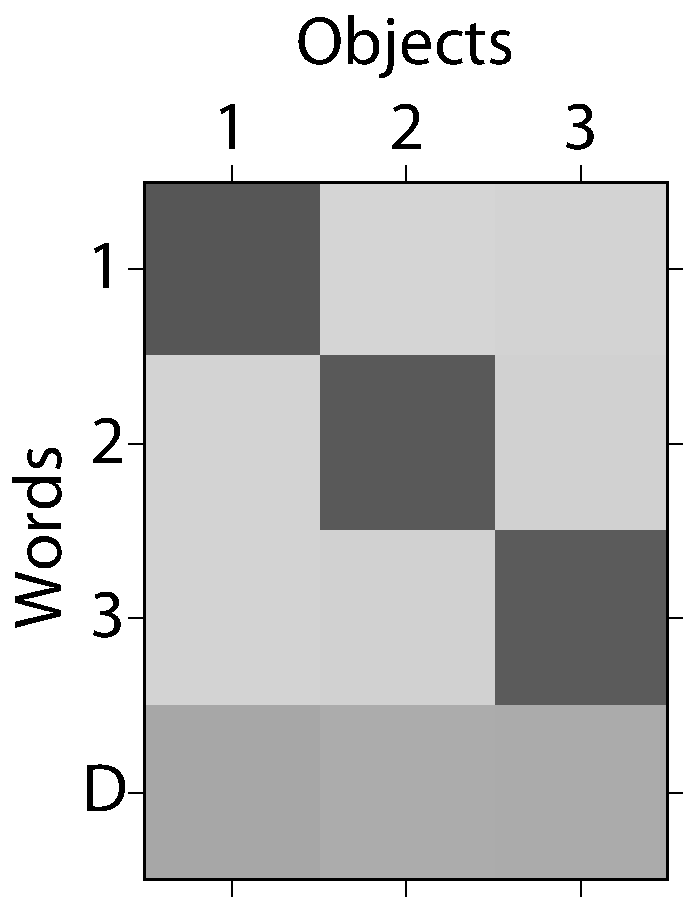
\includegraphics[width=0.2\textwidth]{figures/cross-sit-mod.pdf}
%   \caption{Results from a simulation of cross-situational word learning. The posterior distribution over the learner's lexicon (diagonal entries are correct for word/object pairs 1 -- 3; word D is a distractor). Training data were situations including two of the three objects and a single word, either the distractor or a word matching one of the two objects. Crucially, at no point does the learner observe the meaning of any word; they observe only that a word was produced in each situation.}
%   \label{fig:cross-sit}
% \end{SCfigure}

\section{The role of pragmatics in language acquisition}

\subsection{Disambiguation using known words}

% \begin{SCfigure}[1]
%   \centering
%   % 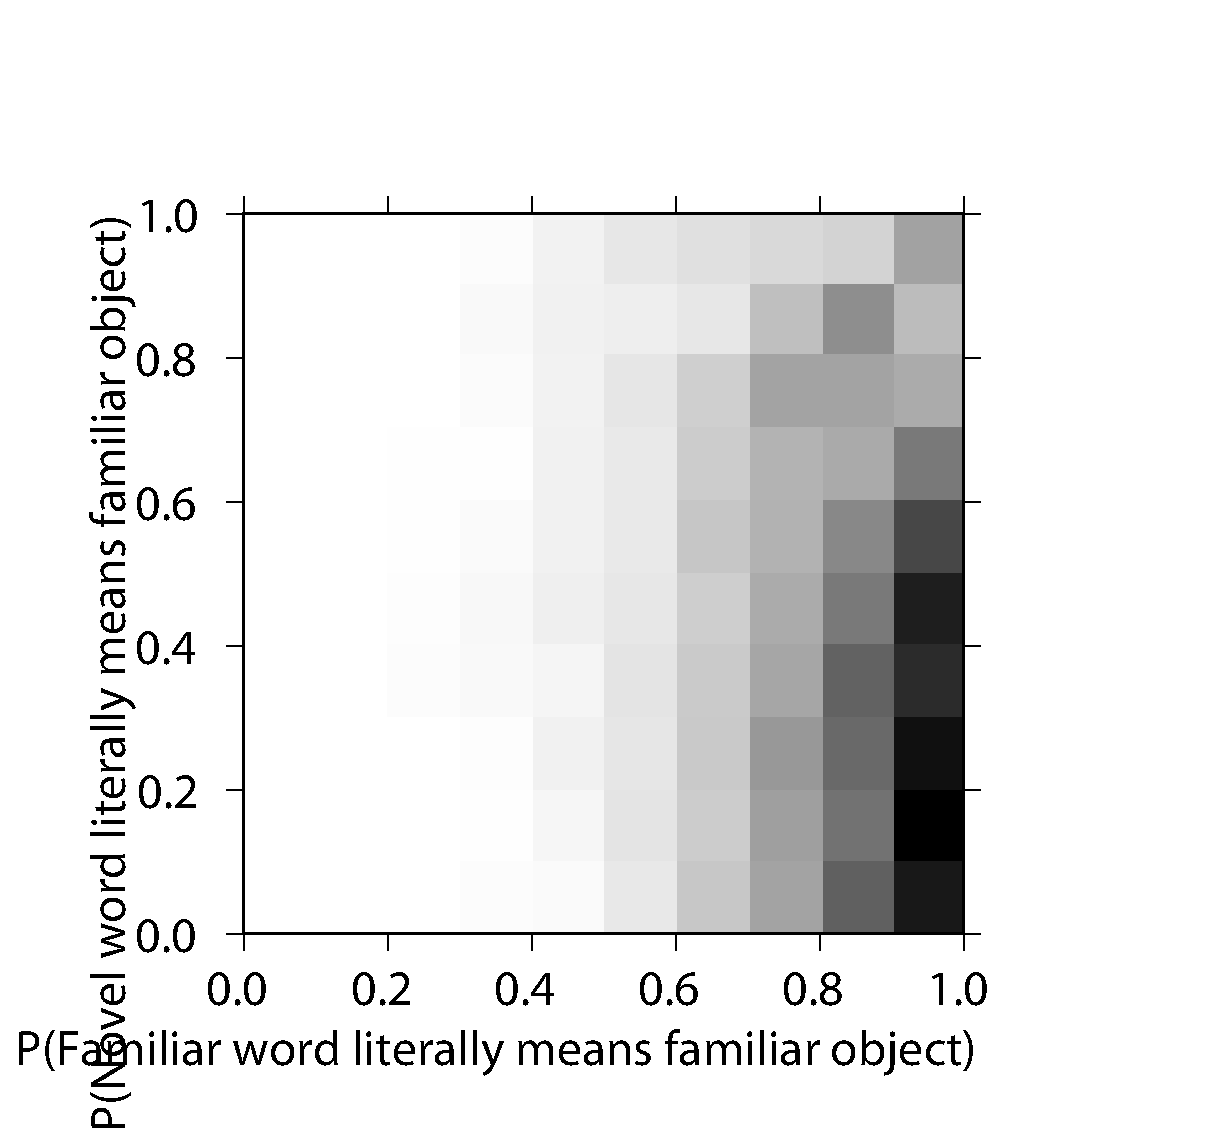
\includegraphics[width=0.24\textwidth]{figures/ME-1dax.pdf}
%   % 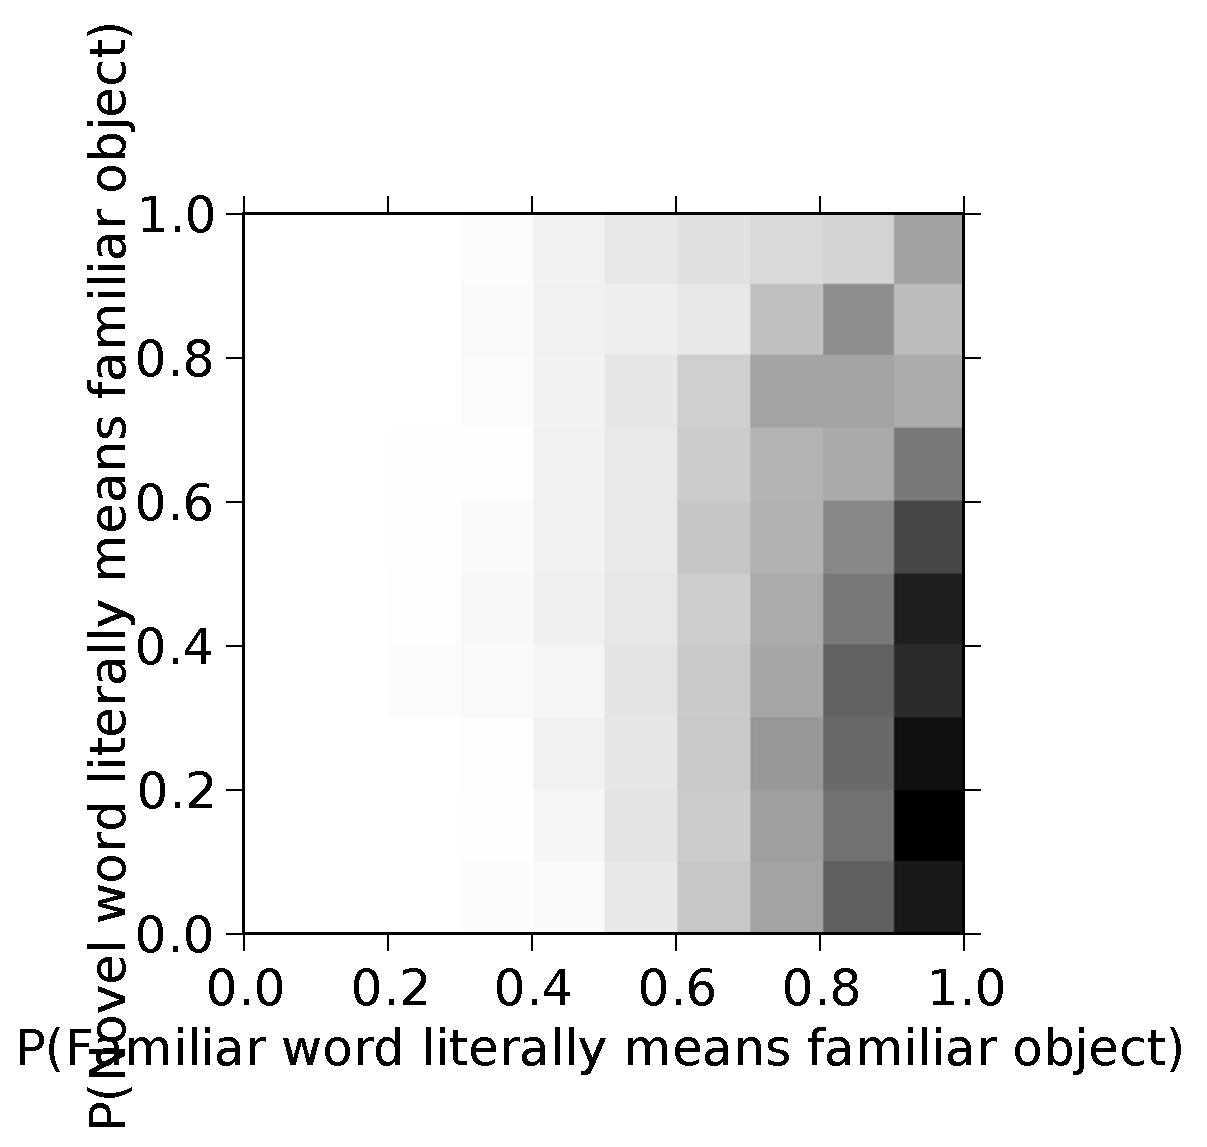
\includegraphics[width=0.24\textwidth]{figures/ME-flat-10dog-10dax.pdf}
%   % 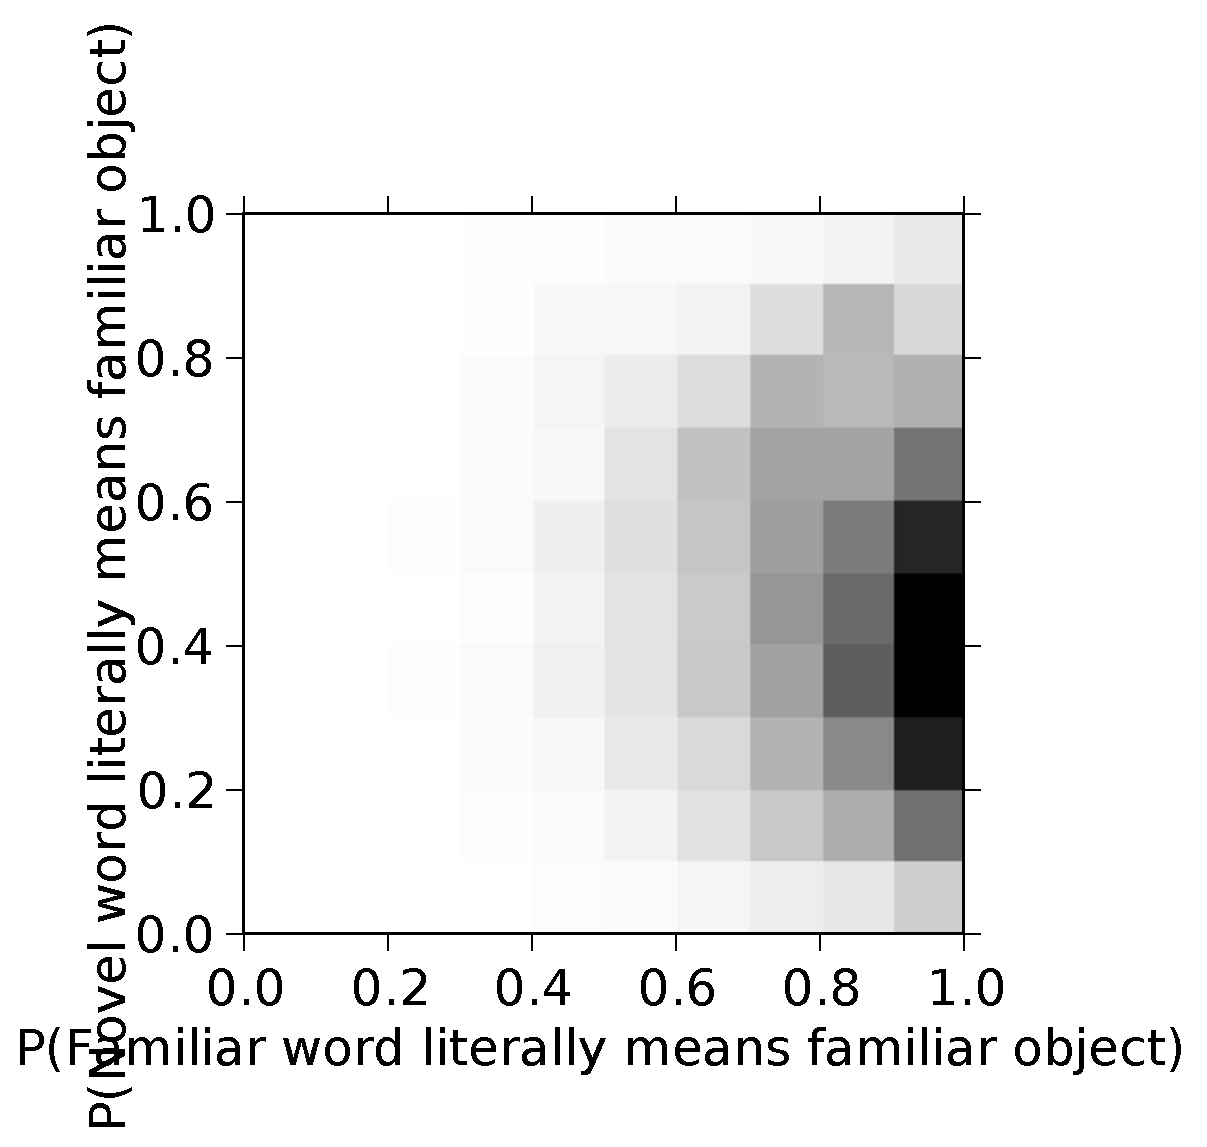
\includegraphics[width=0.24\textwidth]{figures/ME-antisparse-10dog-10dax.pdf}
%   % 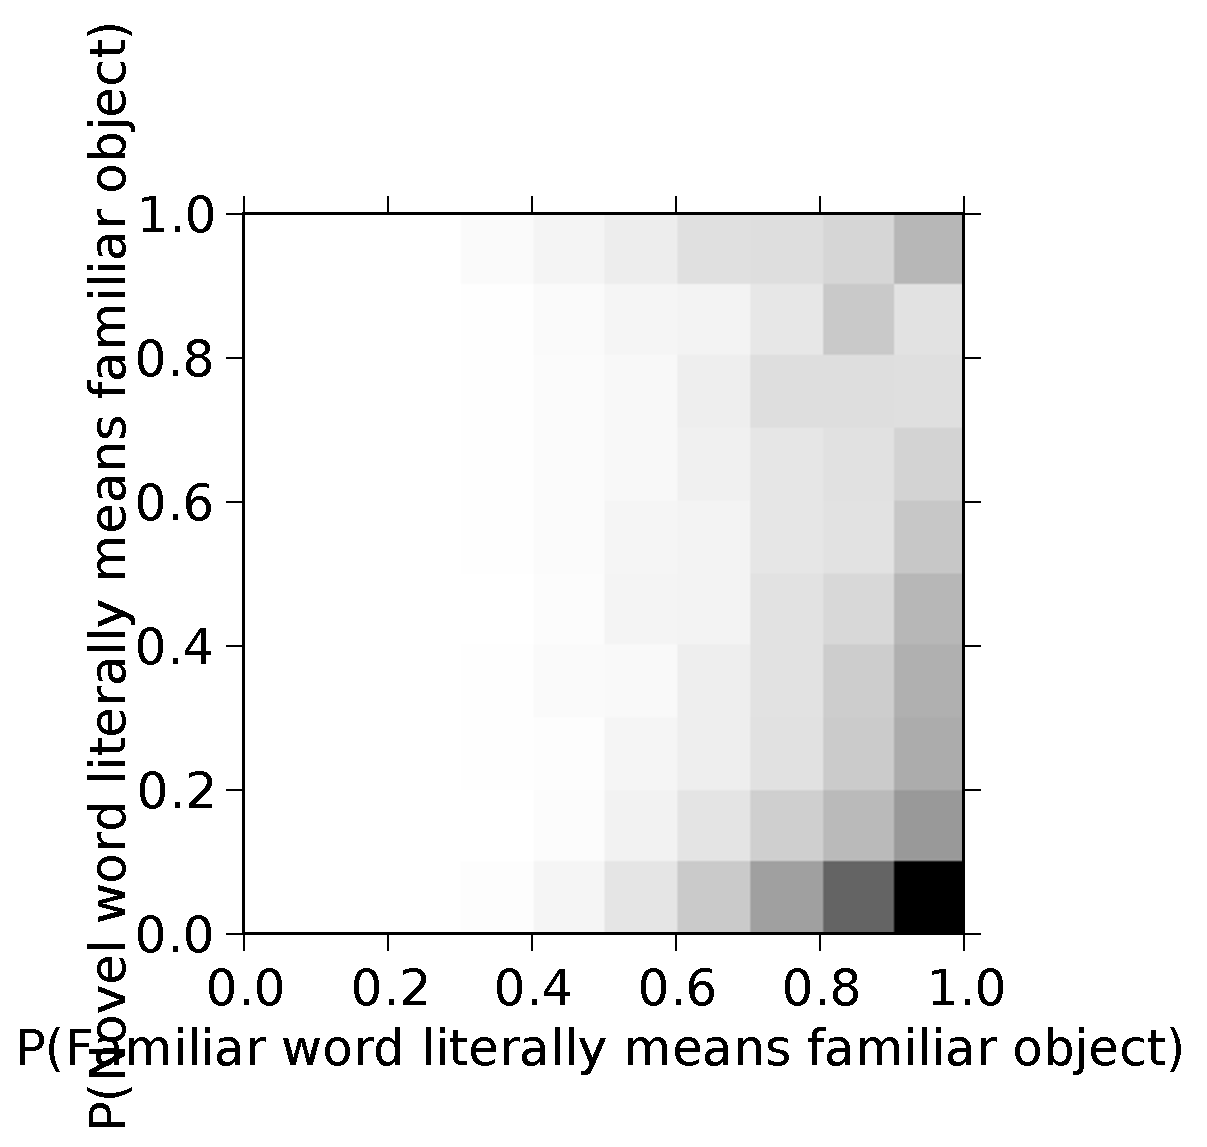
\includegraphics[width=0.24\textwidth]{figures/ME-sparse-10dog-10dax.pdf}
% 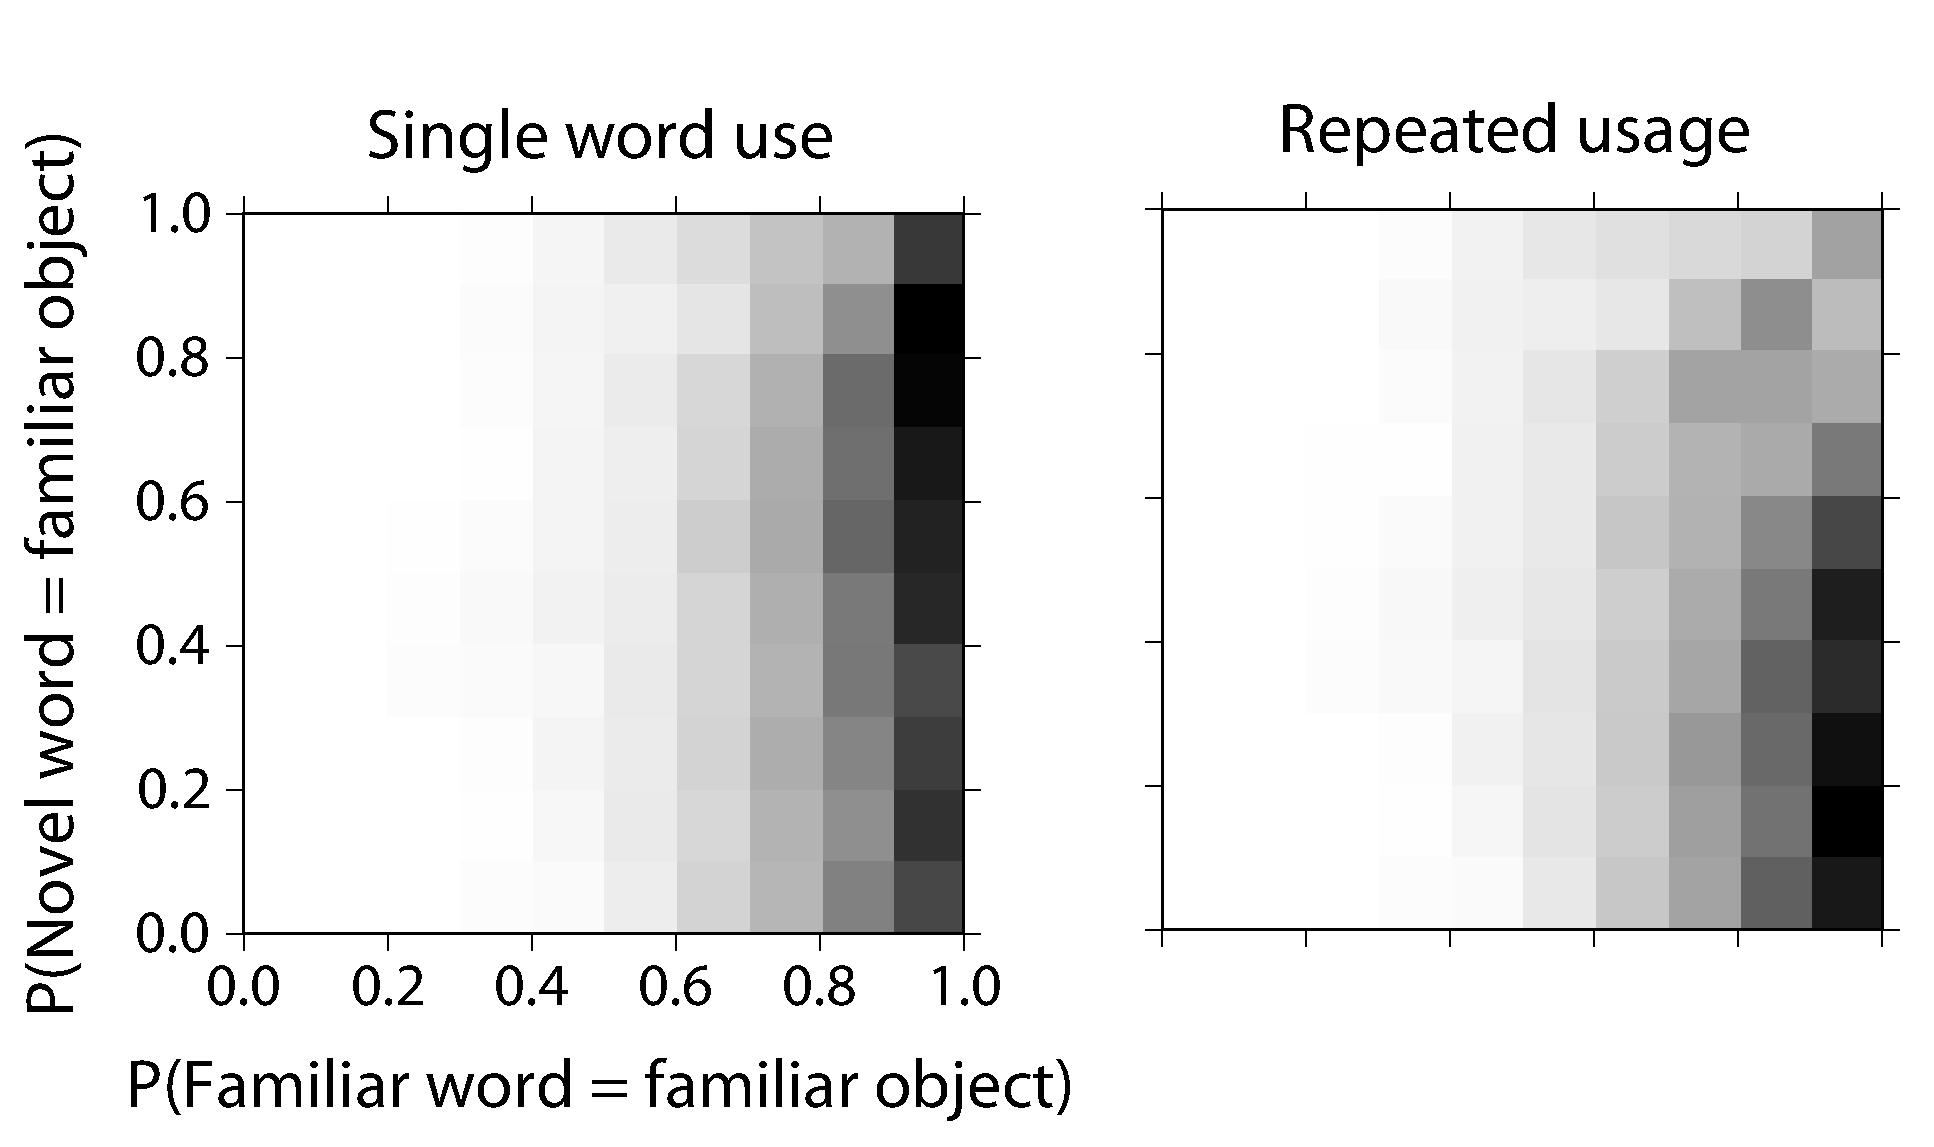
\includegraphics[width=.6\textwidth]{figures/ME-composite-small.pdf}
%   \caption{Results for simulations of the ``disambiguation'' phenomenon. A novel word is used in a situation with a novel object and a familiar object. Each plot shows the joint posterior probability that the familiar word refers to the familiar object (horizontal) and that the novel word refers to the familiar object (vertical). Left plot shows the posterior after a single situation; right plot shows multiple situations.
% %The right middle plot shows the posterior after a single situation given either a prior that makes it likely that there are words referring to both the novel and familiar objects (perhaps because the two objects are physically similar; the right plot shows a situation where the prior makes it unlikely that a word refers to both (objects dissimilar). 
%   }
%   \label{fig:me}
% \end{SCfigure}

Children, when presented with both a novel and a familiar object
(e.g.~an eggbeater and a ball), will treat a novel label
(e.g.~``dax'') as referring to the novel object, for example by
supplying the eggbeater when asked to ``give me the dax''
\cite{markman1988}. This phenomenon is sometimes referred to as
``mutual exclusivity'' or even ``fast mapping.'' Simple probabilistic word learning models can produce a
similar pattern of findings \cite{frank2009}, but all such models assume that learners retain the
mapping between novel word and novel object demonstrated in the
experimental situation. This observation is contradicted, however, by
evidence that children often do not retain the mappings that are
demonstrated by their inferences in the moment \cite{horst2008}.

Our model provides an intriguing possible explanation of this finding:
given a single disambiguation situation, the model gives a substantial
probability (e.g.~75\%) that the speaker is referring to the novel
object. Nevertheless, this inference is not accompanied by an increased belief
that the novel word literally refers to this object. The learner's
interpretation arises not from lexical mapping but instead from a kind
of 
specificity implicature: the listener knows that the familiar word
\emph{does not} refer to the novel object---hence the novel word (even
if it refers to the familiar object as well) is the best way to refer
to the novel object. Nevertheless, on repeated exposure to the same
novel word, novel object situation, the learner does learn the mapping
as part of the lexicon (congruent with other data on repeated training
on disambiguation situations \cite{bion2012}).

% Novel word means: Familiar object: 25.5%. Novel object: 74.5%.
% To anti-sparse listener, novel word means: Familiar object: 21.4%. Novel object: 78.6%.
% To sparse listener, novel word means: Familiar object: 30.5%. Novel object: 69.5%.

\subsection{Preservation of specificity implicatures}
\label{sec:learning-specificity-implic}

% \begin{SCfigure}[1]
% \centering
% 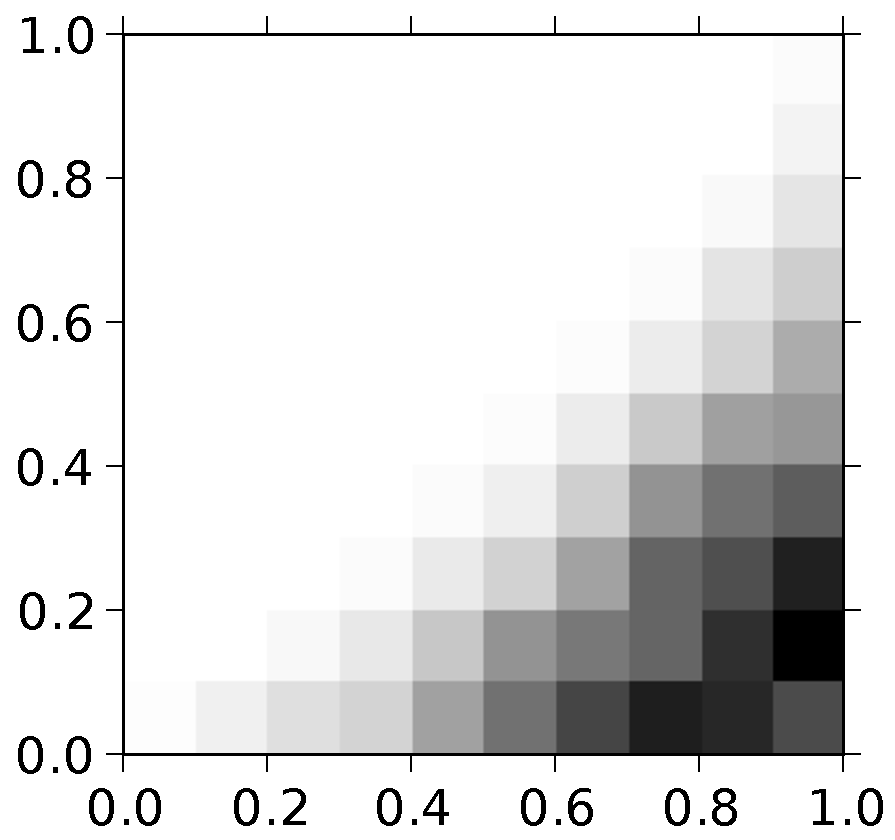
\includegraphics[width=1.5in]{figures/some-all-only-pragmatic.pdf}
% 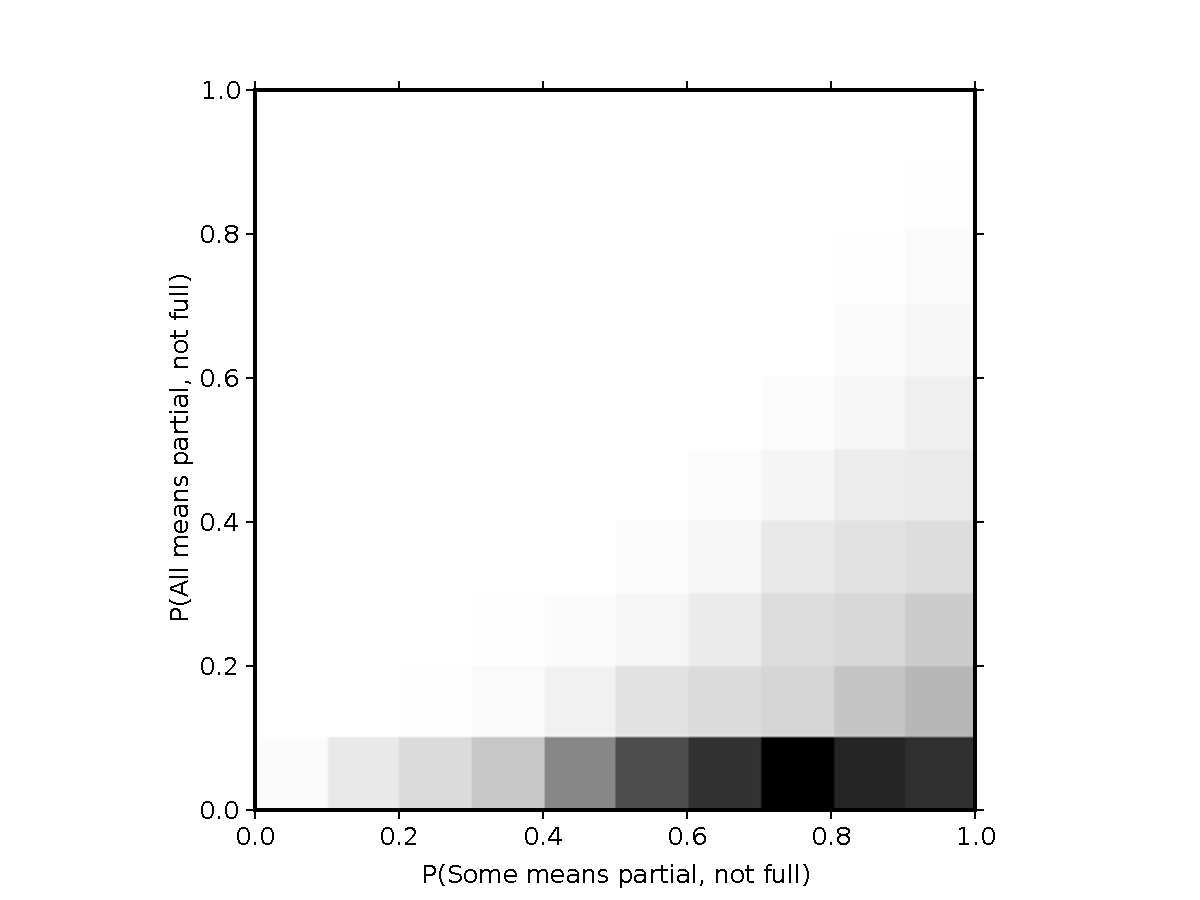
\includegraphics[width=1.5in]{figures/some-all-pragmatic+unambiguous.pdf}
% \caption{\label{fig:scalar} Simulations..}
% \end{SCfigure}

% XX on figure, add x label: ``some'' means: ALL   SOME   SBNA, y label: ``all'' means: ALL  SOME  SBNA

The acquisition of scalar adjectives like ``some'' provides a puzzle
for most models of word learning: given that in many contexts, the
word ``some'' is used to mean \textsc{some-but-not-all}, how do
children learn that {\sc some-but-not-all} is not in fact its literal meaning? Our model
is able to take specificity implicatures into account when learning,
and thus provide a potential solution, congruent with the observation
that no known language in fact lexicalizes {\sc some-but-not-all}.


\begin{figure}[t]
\centering
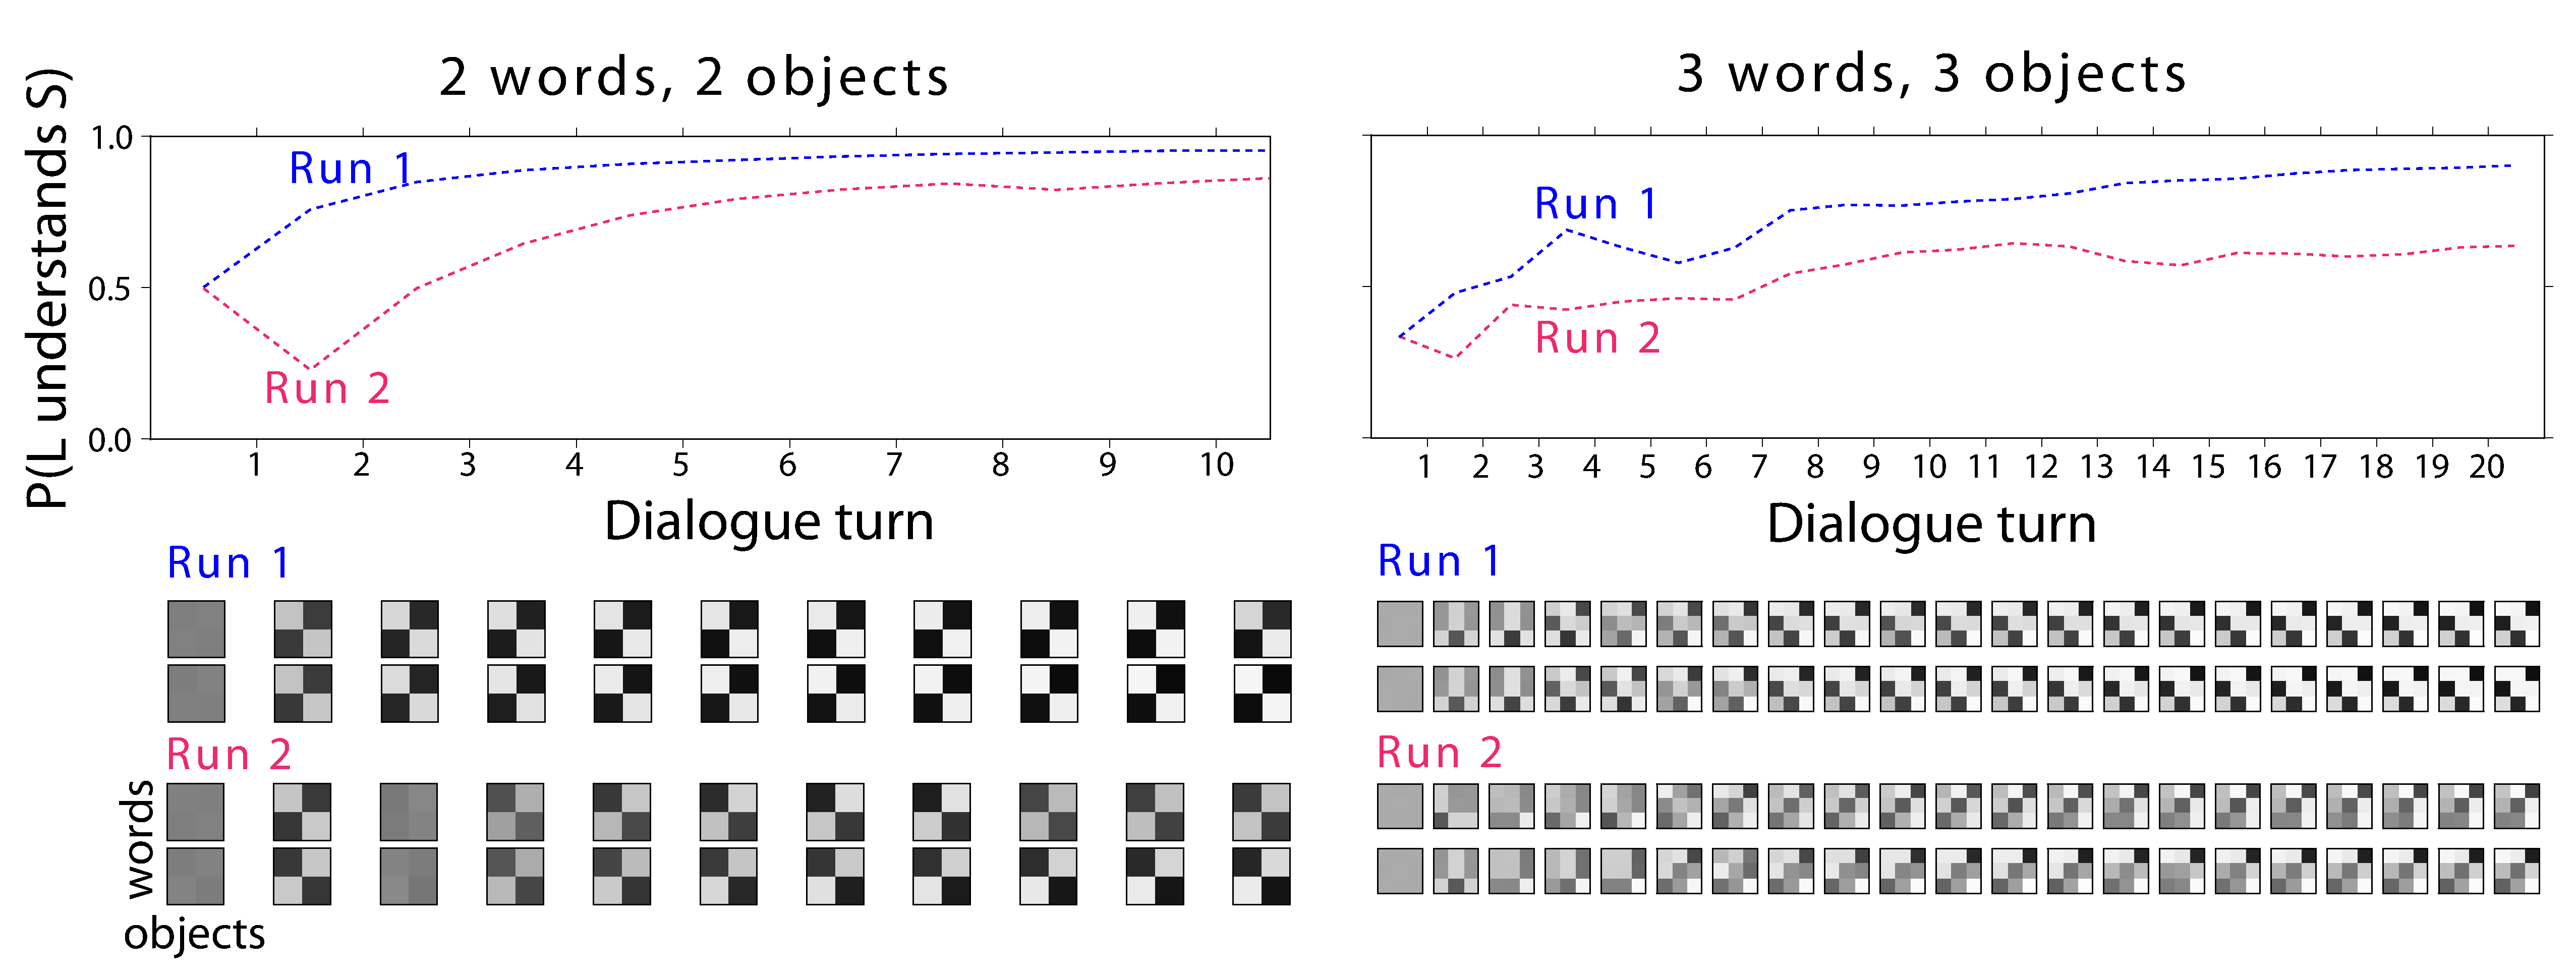
\includegraphics[width=0.98\textwidth]{figures/emergence-composite.pdf}
% 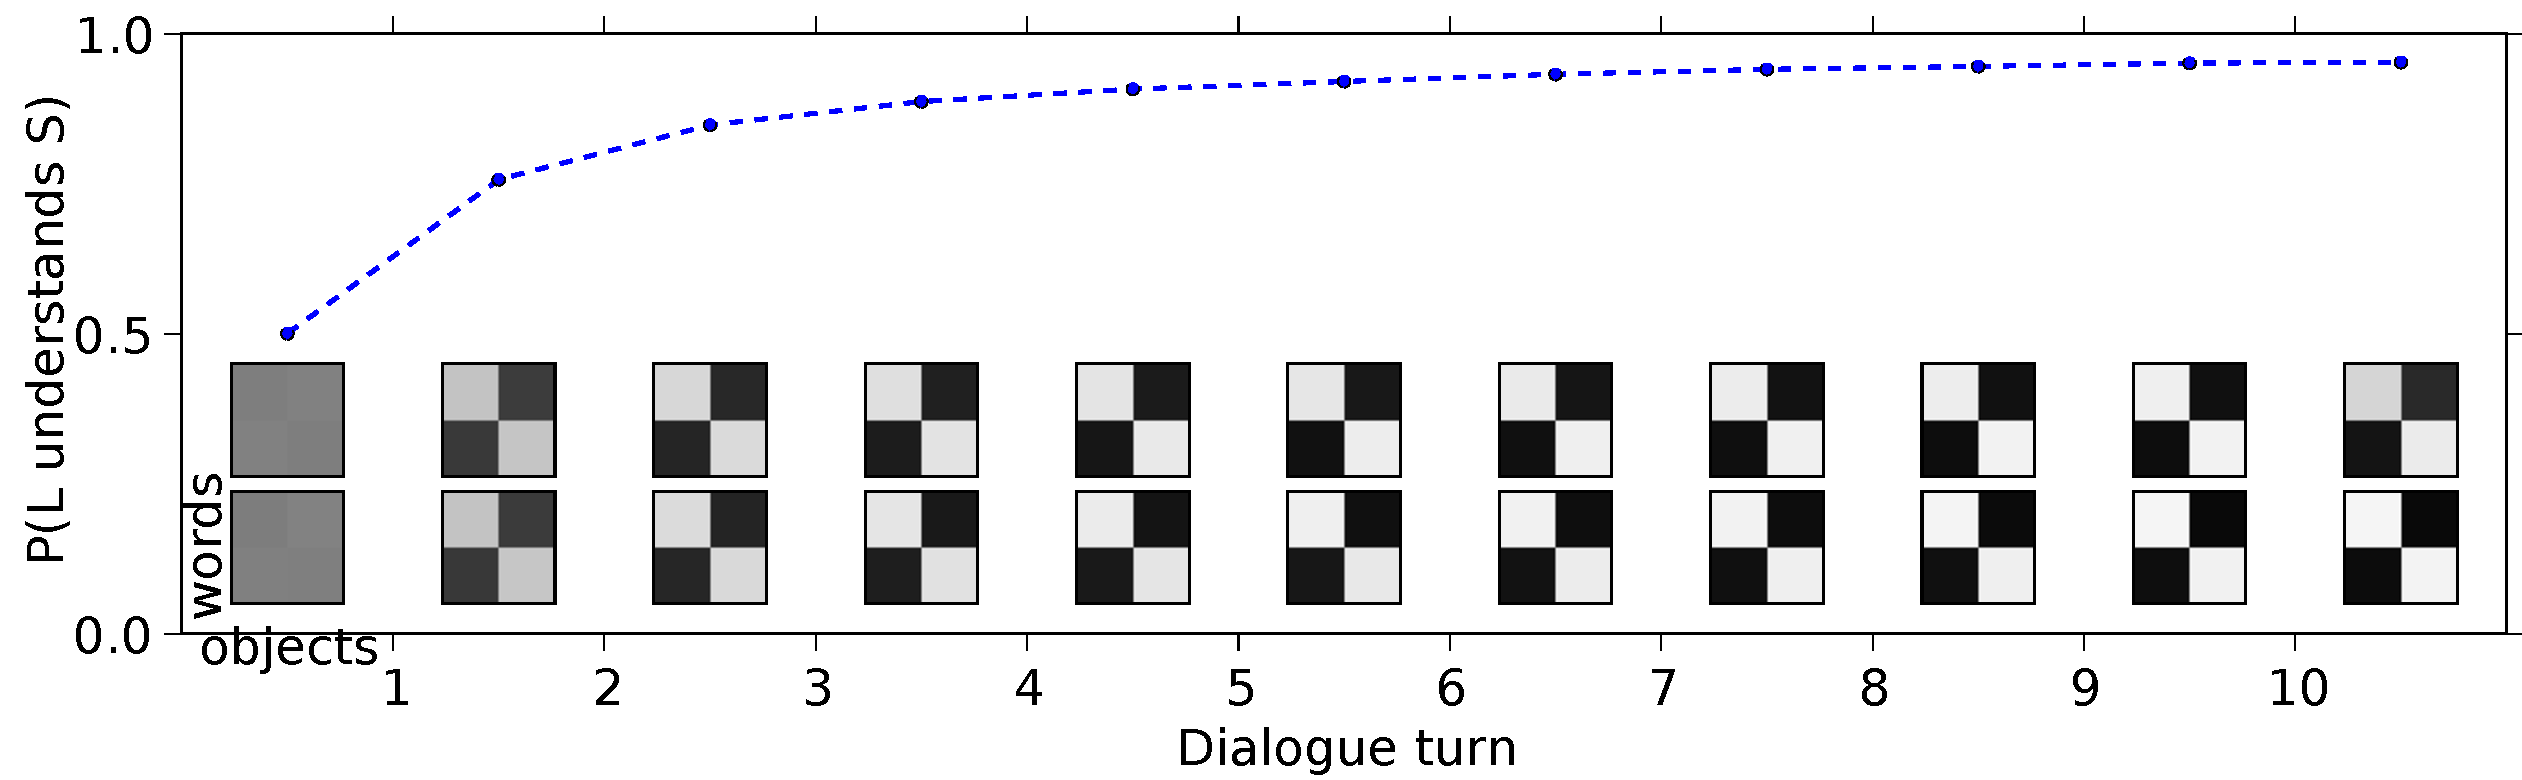
\includegraphics[width=0.48\textwidth]{figures/emergence2x2-1.pdf}
% 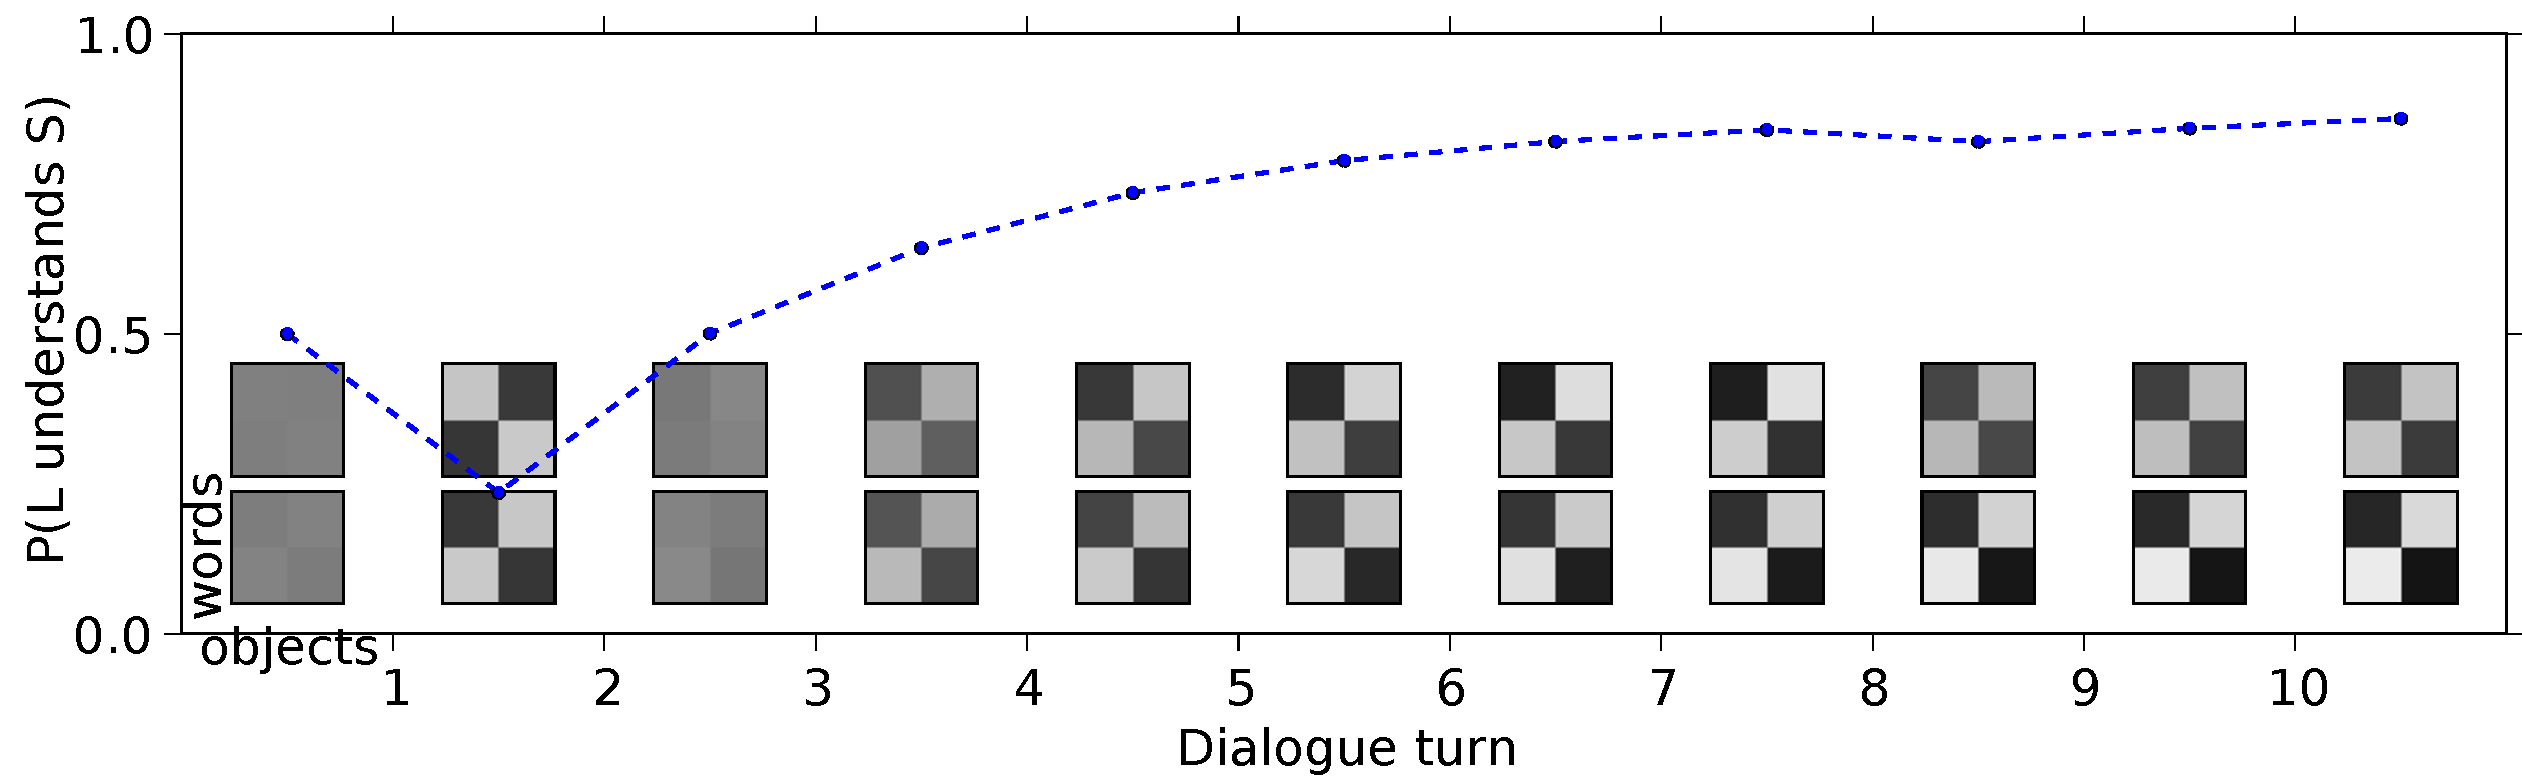
\includegraphics[width=0.48\textwidth]{figures/emergence2x2-3.pdf} \\
% 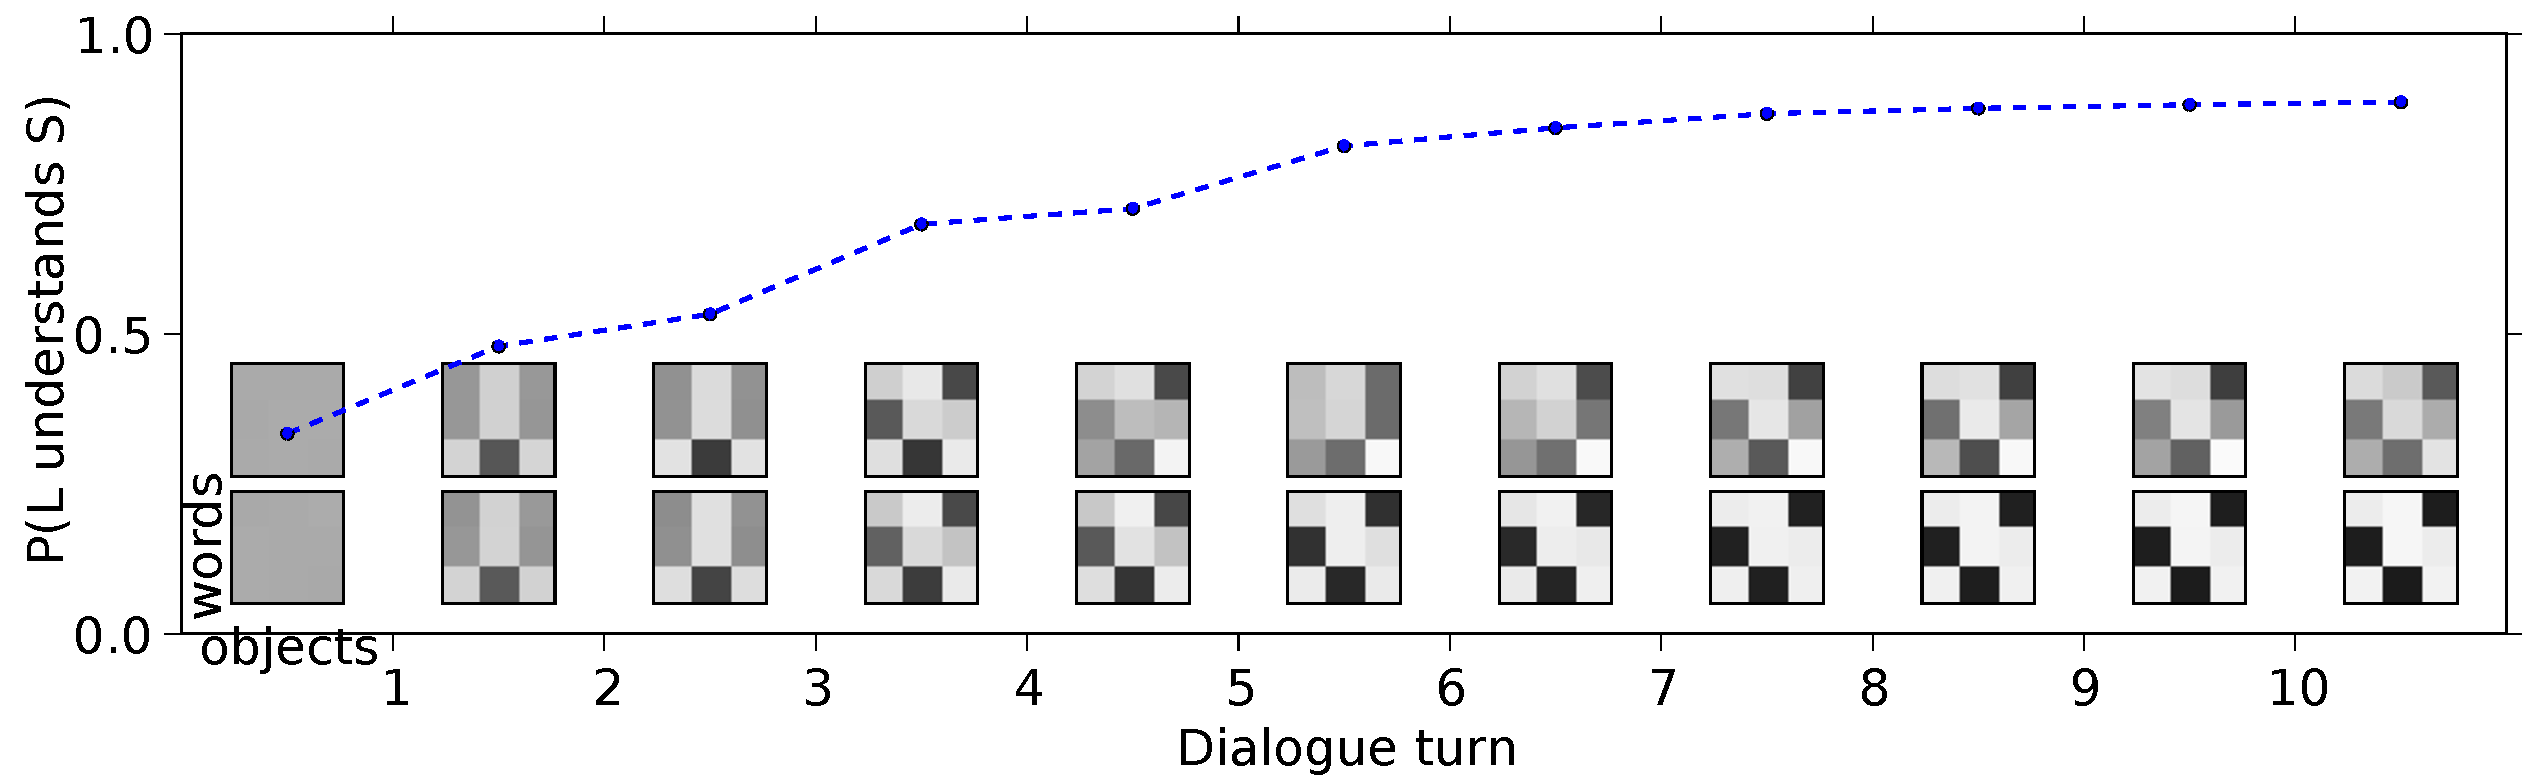
\includegraphics[width=0.48\textwidth]{figures/emergence3x3-0.pdf}
% 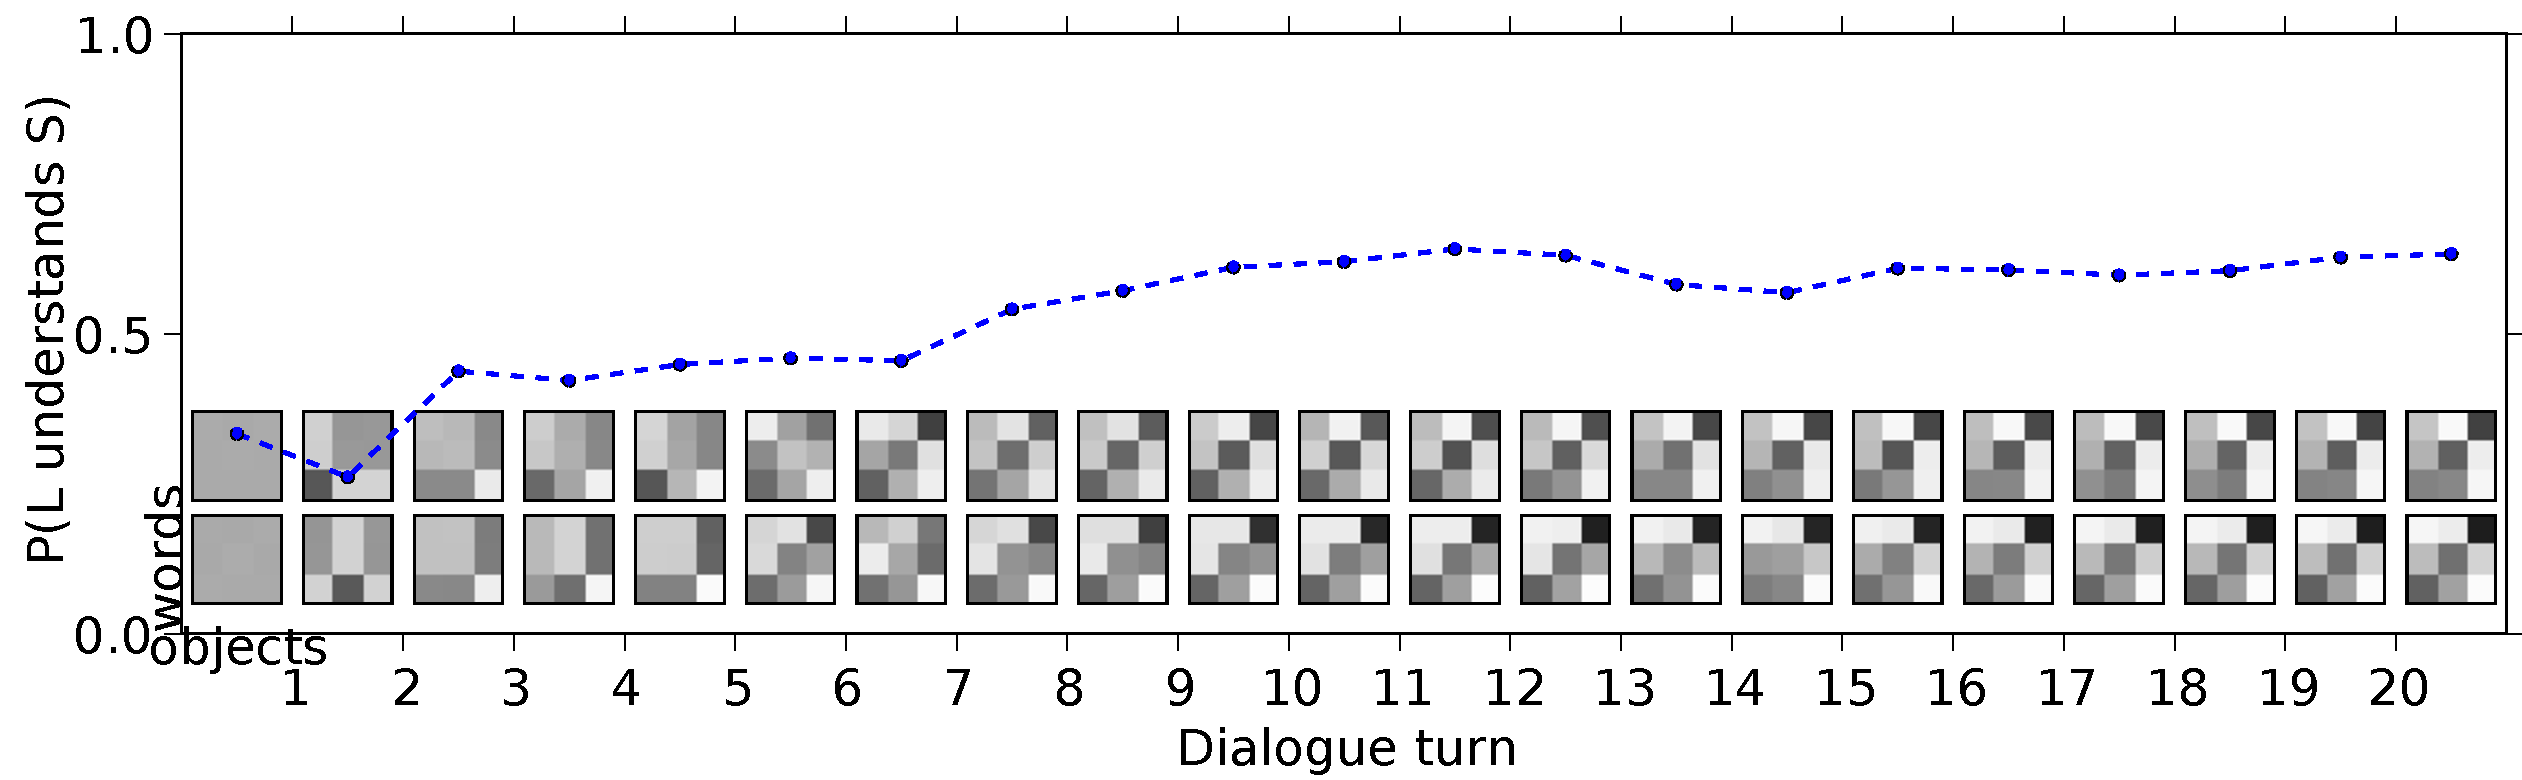
\includegraphics[width=0.48\textwidth]{figures/emergence3x3-1.pdf} \\
\caption{\label{fig:emergence} Simulations of two pragmatic agents
  playing a naming game. Each panel shows two representative
  simulation runs, with run 1 chosen to show strong convergence and
  run 2 chosen to show relatively weaker convergence. At each stage,
  $S$ and $L$ have different, possibly contradictory posteriors over
  the conventional, consensus lexicon. From these posteriors we derive
  the probability $P(\text{$L$ understands $S$})$ (marginalizing over
  target objects and word choices), and also depict graphically $S$'s
  model of the listener, $P_{L_n}(\obj | \word, \text{$S$'s data})$
  (top row within each run),
  and $L$'s actual model, $P_{L_n}(\obj | \word, \text{$L$'s
    data})$ (bottom row within each run). }
\end{figure}

Following the details of \S\ref{sec:spec}, we created a simulation in
which the meaning of ``all'' was fixed to be a particular set {\sc
  all}, and where the learner must infer the meaning of ``some,''
distinguishing two possible meanings: {\sc some-but-not-all}
(unambiguous, 
pragmatically strengthened) or
{\sc some-but-not-all or all} (ambiguous). Training exposure in the
simulation consisted of situations in which ``some'' was pragmatically
strengthened to refer to {\sc some-but-not-all}. Despite this
unambiguous training, the model maintained substantial
posterior probability on the correct (ambiguous) hypothesis about the
meaning of ``some.'' In each
situation, the model essentially reasoned that although the evidence
was unambiguous, it could have been produced by an implicature and
hence should be discounted. Thus, a pragmatically-informed learner
might both be able to maintain the true meaning of {\sc some} and
interpret it correctly as denoting {\sc some-but-not-all} in
appropriate contexts. 


% Exposure to these
% situations does not result in mapping of ``some'' to {\sc
%   some-but-not-all}, despite the evidence that 
% Imagine two bowls: one
% containing a mixture of apples and oranges, the other containing
% apples alone. After encountering the words ``some'' and ``all'' used contrastively
% to refer to these two bowls (as in e.g.\ ``the bowl with some
% apples''), a learner under our model believes that at least one of these words must have a
% restrictive literal meaning, but not both---it leaves open the
% possibility that either ``some'' or ``all'' might be literally
% ambiguous. But if examples of ``some'' are given that refer to exactly
% the same object in contexts where this is the only object
% available, so there is no contrast and thus no implicature; this
% convinces the model that ``all apple'' literally refers only to the
% bowl that contains no oranges, while ``some'' most likely is somewhat
% ambiguous. Crucially, the model is able to learn this without once
% ever observing ``some'' used

% s1: reasonable chance that ``some'' literally refers to only one, but
% maybe ``some'' refers to both. so you can learn ambiguity even with
% unambiguous evidence. 

% s2: 

% agents not sure whether some literally means some-not-all or not,
% could lexicalize given the right kind of input, but regular pragmatic
% strengthening alone is not enough

\section{Mutual learning situations}


\subsection{Emergence of efficient communicative conventions}
\label{sec:emergence}

Experimental results suggest that communicators are able to establish
novel, consensus-based communication systems. For example, adults
playing a communication game using only novel symbols with no
conventional meaning will typically converge on a set of new
conventions which allow them to accomplish their task
\cite{galantucci2005}. Or in a less extreme example, communicators
asked to refer to novel objects invent conventional names for them
over the course of repeated interactions (e.g., ``the ice skater'' for
an abstract figure vaguely resembling an ice skater,
\cite{clark1986}). From a pure learning perspective this behavior is anomalous,
however: Since both agents know perfectly well that there is no
existing convention to discover, there is nothing to learn from the
other's behavior. Furthermore, even if only one partner is producing
the novel expressions, their behavior still becomes more regular
(conventional) over time, which would seem to rule out a role for
learning---even if there is some pattern in the expressions the
speaker chooses to use, there is certainly nothing for the
\textit{speaker} to learn by observing these patterns, and thus their
behavior should not change over time.
% An obvious hack might be to simply stipulate that speakers take
% their own utterances as training data for further learning, but this
% would fail to explain yet another wrinkle in this phenomenon:
% speakers only regularize their production over time if they have
% some kind of feedback indicating that the listener understands; if
% such feedback is removed, the phenomenon is dramatically reduced (X X
% krauss 1966, branigan catchpole pickering 2011).


To model such phenomena, we imagine two agents playing the simple
referential game introduced above. On each turn the speaker is
assigned a target object, utters some word referring to this object,
the listener makes a guess at the object, and then, critically, the
speaker observes the listener's guess and the listener receives
feedback indicating the correct answer (i.e., the speaker's intended
meaning). The listener then updates their posterior over lexicons
before proceeding to the next trial. As in
\cite{krauss1964,clark1986}, the speaker and listener remain fixed in
the same role throughout.

Fig.~\ref{fig:emergence} shows the result of simulating several such
games when both parties begin in total ignorance. Notice that: (a)
agents' performance begins at chance, but quickly rises; (b) they tend
towards structured, sparse lexicons with a one-to-one correspondence
between objects and words; and (c) as the speaker and listener have
entirely different data (the listener's interpretations and the
speaker's intended meaning, respectively), unlucky early guesses can
lead them to believe in entirely contradictory lexicons---but they
generally recover and converge. Each agent effectively uses their
partner's behavior as a basis for forming weak beliefs about the
underlying lexicon that they assume must exist. Since they then each
act on these beliefs, and their partner uses the resulting actions to
form new superstitions, they soon converge on using similar lexicons,
and what started as a ``superstition'' becomes normatively correct.
% On the other hand, if the speaker is not allowed to observe the
% listener's guess, then the speaker does no learning and their
% posterior over lexicons remains perfectly uniform. They therefore
% choose words by simply flipping a coin, and performance remains at
% chance.

% Pragmatic inference here does two things. First, the pragmatic
% recursion makes it possible for the speaker to learn from the
% listener's interpretations, which would be impossible without an
% explicit model of the listener as a rational agent. Second, pragmatics
% creates the sparse structure in the observed lexicons: At each step,
% the goal-directed speaker attempts to exploit whatever communicatively
% useful asymmetries exist in its current model of the listener, and
% these attempts tend to be successful. If the listener has even a small
% asymmetry in their current posterior then their pragmatic reasoning
% will magnify it as well.

% But over time, the speaker's use of such patterns, and the
% listener's ability to understand them, will each be taken by the
% other as evidence that these patterns actually exist in the literal
% lexicon. The result is that while both agents start out with uniform
% priors over the lexicon, they are biased to end up believing in
% lexicons that are communicatively useful for the task at hand.

% X X X X what can we say about the role pragmatics plays here? It's
% annoyingly non-trivial to sample from the equivalent model where the
% speaker just samples from a multinomial distribution and the
% listener inverts it. The listener's data is samples from a DM so
% they have conjugacy. But the speaker's data is listener
% interpretations, which necessarily do one tiny pragmatic inference
% step from using Bayes rule, which breaks conjugacy...

\subsection{Lexicalization and loss of Horn implicatures}
\label{sec:horn-emergence}


\begin{SCfigure}
\centering
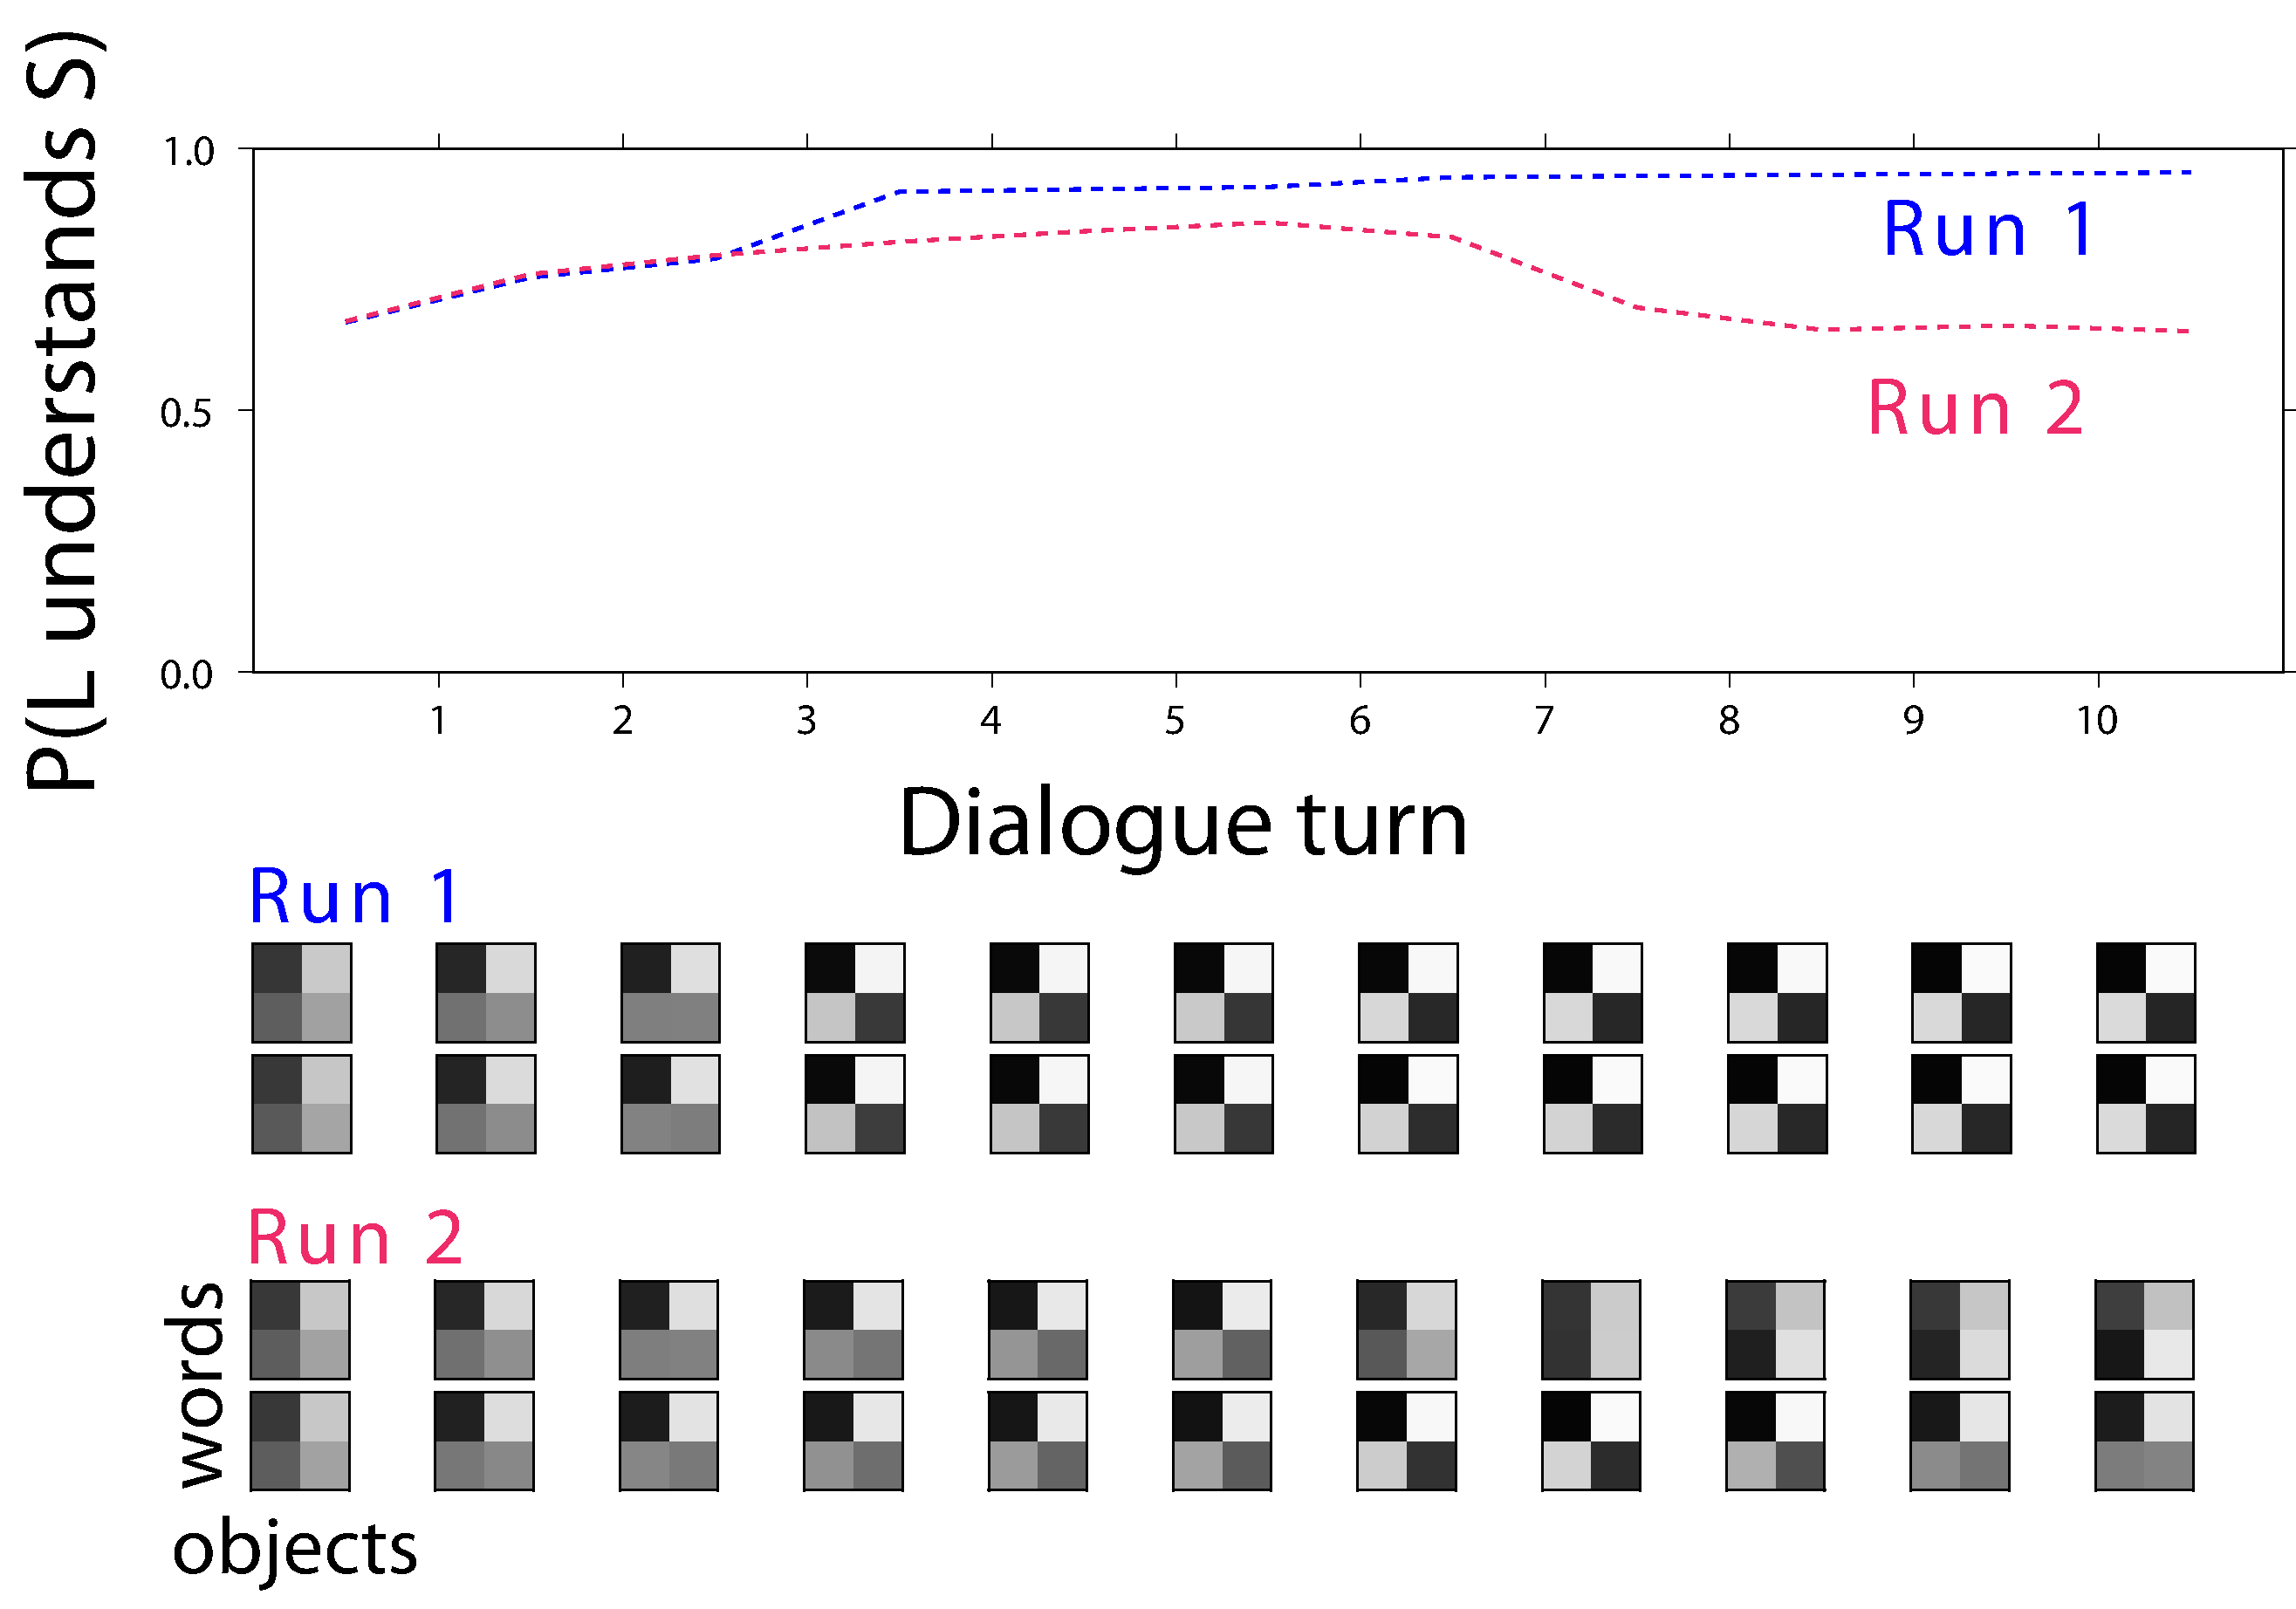
\includegraphics[width=0.5\textwidth]{figures/horn-composite.pdf}
% 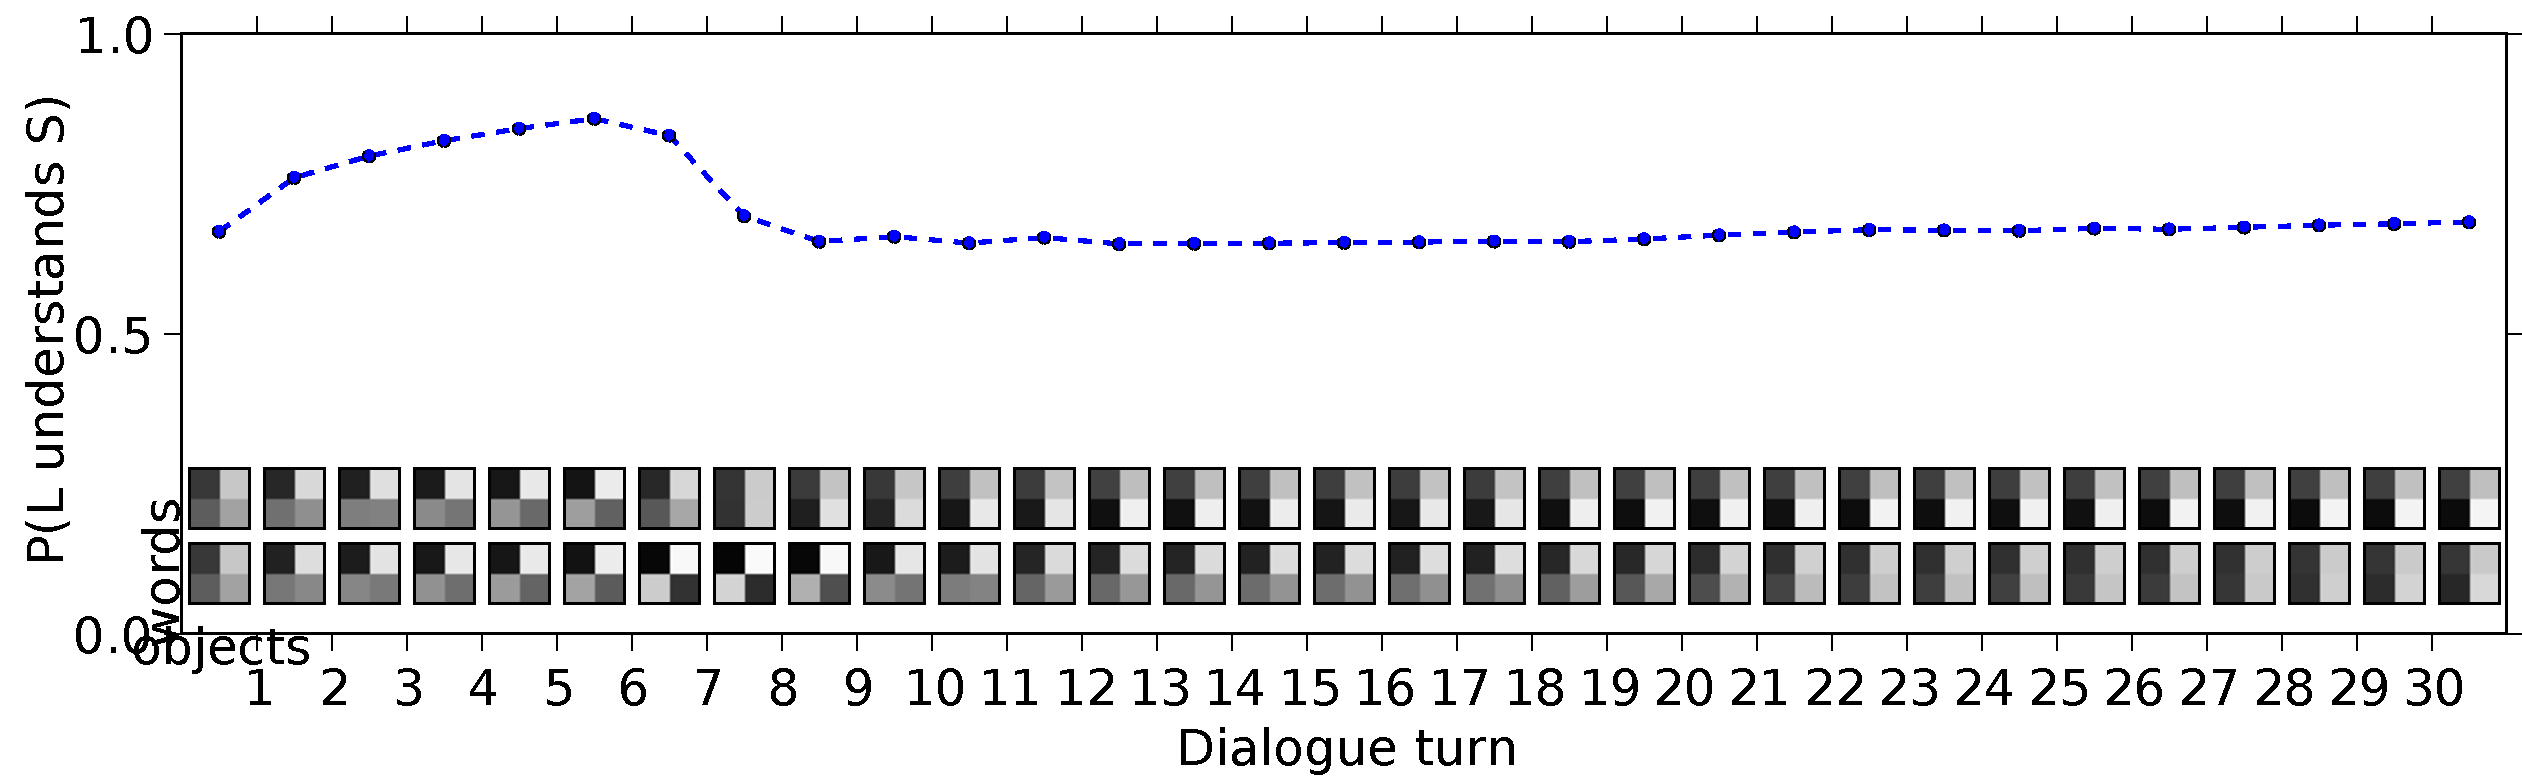
\includegraphics[width=0.48\textwidth]{figures/horn-emergence-1.pdf}
\caption{\label{fig:horn} Example simulations showing the
  lexicalization of Horn implicatures. Plotting conventions are as
  above. In the first run, speaker and listener converge on a sparse
  and  efficient communicative equilibrium, while in the second they reach
  a sub-optimal equilibrium.}
\end{SCfigure}



\begin{SCfigure}
\centering
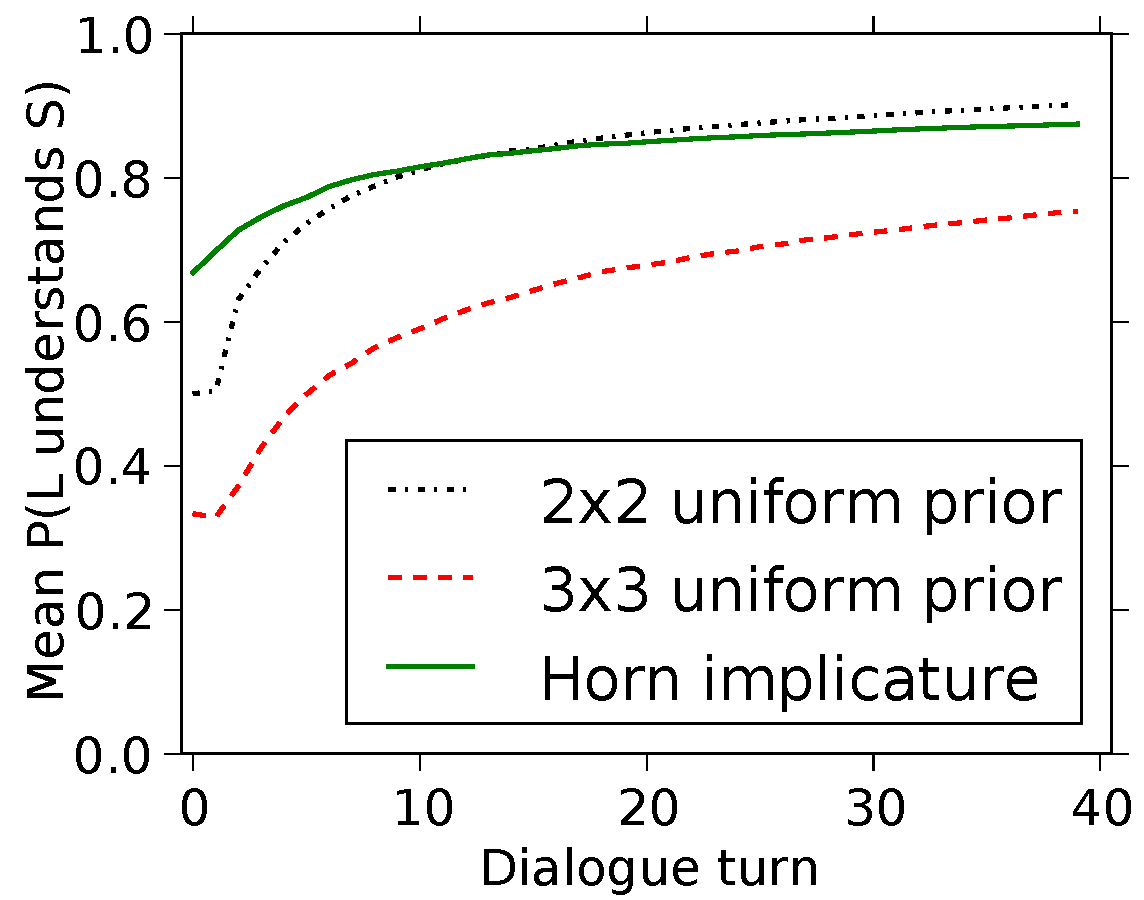
\includegraphics[width=0.3\textwidth]{figures/emergence-average.pdf}
\hspace{0.2in}
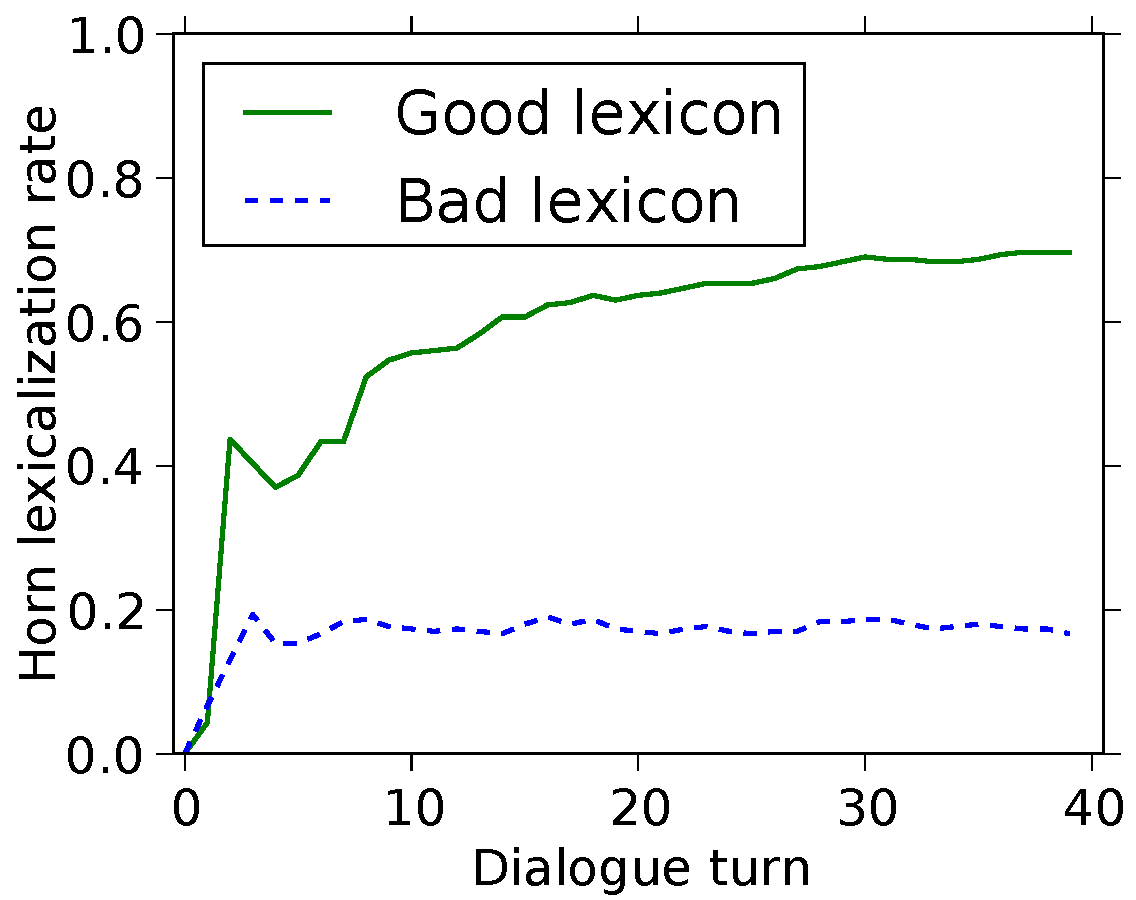
\includegraphics[width=0.3\textwidth]{figures/emergence-horn-average.pdf}
\caption{\label{fig:emergence-average} Averaged behavior over 300
  dialogues as in Figs.~\ref{fig:emergence} and \ref{fig:horn}. Left:
  Communicative success by game type and dialogue turn. Right:
  Proportion of dyads in the Horn implicature game
  (\S\ref{sec:horn-emergence}) who have converged on the ``good'' or
  ``bad'' lexicons and believe that these are literal meanings.}
\end{SCfigure}

A stronger example of how pragmatics can create communicative biases can be
observed by considering the Horn implicatures introduced in \S\ref{sec:horn-implicature}. 
In these games, pragmatic reasoning causes each agent to start out weakly biasedtowards the associations ``cheap'' $\leftrightarrow$
\textsc{common}, ``expensive'' $\leftrightarrow$ \textsc{rare}; this bias arises because their prior on literal meaning
is uniform and uninformative. A fully rational listener, therefore,
observing an uncertain speaker using this mapping, would discount it
as arising from this bias, and conclude that the speaker in fact did
not know which convention was in use. Conventional listeners,
however, believe that speakers do know which convention is in
use, and therefore tend to take their behavior as positive evidence that the
``good'' system is in use. Similarly, conventional speakers
will wager that since on average they will succed more often if
listeners are using the ``good'' system, they might as well try
it. When they succeed, they take their success as evidence that the listener was in
fact using the good system all along. As a result, dyads in this game
 end up converging onto a stable system at a rate far above
chance (Fig.~\ref{fig:horn}). 

Something
fundamentally different happens in this case than in the specificity
implicature case (\S\ref{sec:learning-specificity-implic}), however. There, we
saw that our model could hear pragmatically strengthened usages
of words while recovering the underlying literal meaning. In the Horn
case, though, the pragmatic strengthening depends essentially on
ignorance about literal meaning. As the agents gather more data,
the implicature disappears, to be replaced by a belief that
``cheap'' \textit{literally} means \textsc{common}. To demonstrate
this phenomenon, we queried each agent in each dyad about how they would refer to
or interpret each object and word, \textit{if} the two objects were
equally common, which cancels the Horn implicature. As shown in
Fig.~\ref{fig:emergence-average} (right), after 30 turns, in nearly 70\%
of dyads both $S$ and $L$ believed in the ``good'' mapping even in
this implicature-free case, while less than 20\% believed in the
``bad'' mapping (with the rest being inconsistent). This makes the
interesting prediction that while specificity implicatures can survive
indefinitely in a language system, any Horn implicatures that arise
consistently should transition to becoming part of the literal meaning
of the words involved.

% To show that they're lexicalized, at end of each of 4 dialogues, we
% look at how speaker and listener talk about/interpret the objects/words:
%
% Dialogue 0, after disabling implicature:
%   How speaker refers to "common" and "rare" objects:
% array([[  9.99994601e-01,   1.67862018e-02],
%        [  5.39888463e-06,   9.83213798e-01]])
%   Listener's interpretation of "cheap" and "expensive" words:
% array([[ 0.84765063,  0.15234937],
%        [ 0.02451694,  0.97548306]])

% Dialogue 1, after disabling implicature:
%   How speaker refers to "common" and "rare" objects:
% array([[  9.99997339e-01,   1.04639034e-02],
%        [  2.66058112e-06,   9.89536097e-01]])
%   Listener's interpretation of "cheap" and "expensive" words:
% array([[ 0.86951534,  0.13048466],
%        [ 0.01986478,  0.98013522]])

% Dialogue 2, after disabling implicature:
%   How speaker refers to "common" and "rare" objects:
% array([[  9.99984637e-01,   2.19135388e-02],
%        [  1.53629560e-05,   9.78086461e-01]])
%   Listener's interpretation of "cheap" and "expensive" words:
% array([[ 0.83486332,  0.16513668],
%        [ 0.03421814,  0.96578186]])

% Dialogue 3, after disabling implicature:
%   How speaker refers to "common" and "rare" objects:
% array([[  9.99996148e-01,   1.92821280e-02],
%        [  3.85172462e-06,   9.80717872e-01]])
%   Listener's interpretation of "cheap" and "expensive" words:
% array([[ 0.83985034,  0.16014966],
%        [ 0.02170542,  0.97829458]])

\section{Conclusion}

Language learners and language users must consider word meanings both
within and across contexts. A critical part of this process is
reasoning pragmatically about agents' goals in individual
situations. In the current work we assume that agents communicating
with one another assume that there is a shared conventional lexicon
which they both rely on. They then
reason recursively about how this lexicon should be used to convey
particular meanings in context. This pair of assumptions allows us to
create a model that unifies two previously separate strands
of modeling work on language usage and acquisition, and account for a
variety of new phenomena. In particular, we consider new
explanations of disambiguation in early word learning and the acquisition of
scalar adjectives, and demonstrate that our model is capable of developing
novel and efficient communicative systems through iterated learning
within the context of a single simulated conversation.

Our work identifies two biases in communicators' behavior: a tendency for pragmatic speakers
and listeners to accentuate useful, sparse patterns in their
communicative systems (\S\ref{sec:emergence}), and for short,
high-frequency (``low cost'') expressions to
be assigned to common objects (\S\ref{sec:horn-emergence}).
Remarkably, while both of these biases are locally sub-optimal for individual agents,
they both systematically drive the overall communicative system
towards greater global efficiency. In the long term, these processes
should leave their mark on the structure of the language itself, which
may contribute to explaining how languages become 
optimized for effective communication \cite{zipf1936,piantadosi2011}.

% the deviations from rationality -- assumption that words have
% meanings, suspicion that everyone else knows what they are -- are
% highly interpretable and intuitively compelling, and while like any
% deviations from rationality they necessarily introduce biases, these
% biases appear in this case to improve the global performance of the
% system.

% if you're trying to collaborate with an agent who soft-maximizes
% utility, but there are multiple possible rules which might underlie
% their utility function, you should assign more weight to those rules
% which provide a sharp distinction in utility for different actions --
% which will generally be the rules that allow for higher expected
% utility. this actually explains both the uniform prior and the horn
% implicature emergence results.

% provides new insight into use of pragmatic reasoning in word learning,
% the learning of literal meanings given pragmatically strengthened
% input, and makes the interesting prediction that some implicatures are
% intrinsically more stable, while others if consistently supported will
% tend to enter the lexicon and become part of the literal meaning of
% the relevant words.

% zipf, piantidosi et al

%\subsubsection*{Acknowledgments}


% Thanks to ONR Grant #blahblah

\newpage
\small
\bibliographystyle{plain}
\bibliography{pragmatics}

\end{document}
